\chapter{Implementation} \label{cpt-implementation}

The implementation used for the experiment is based on an implementation within the framework \emph{Diligent Engine} 
\cite{DiligentGraphicsGitHub, DiligentGraphics}. This framework includes a rendering backend supporting 
multiple rendering \ac{API}s, with integrations for modern \ac{GPU}-driven rendering, such as the support for 
mesh shading in Microsoft's D3D12 rendering \ac{API}. The support for modern rendering features, while still 
maintaining access to all core features, makes \emph{Diligent Engine} a good place to start from.\\

\noindent
For the experiment, the mesh shading pipeline is enhanced to better fit the purpose of drawing a huge amount of voxels. 
Also, the integrated meshlet-based view-frustum culling was altered to some degree so that it works on meshlet-groups 
rather than meshlets themselves. This change was made during the restructuring of the draw tasks. The updated pipeline 
changes how meshes are dispatched because of the use of additional acceleration structures. This chapter provides 
a detailed overview of the complete pipeline and how it works in particular. The full implementation details can be 
found in appendix \ref{cpt-appendix}.

\section{Pipeline Initialization} \label{sec-piepline-initialization}

\begin{figure}[h]
    \centering
    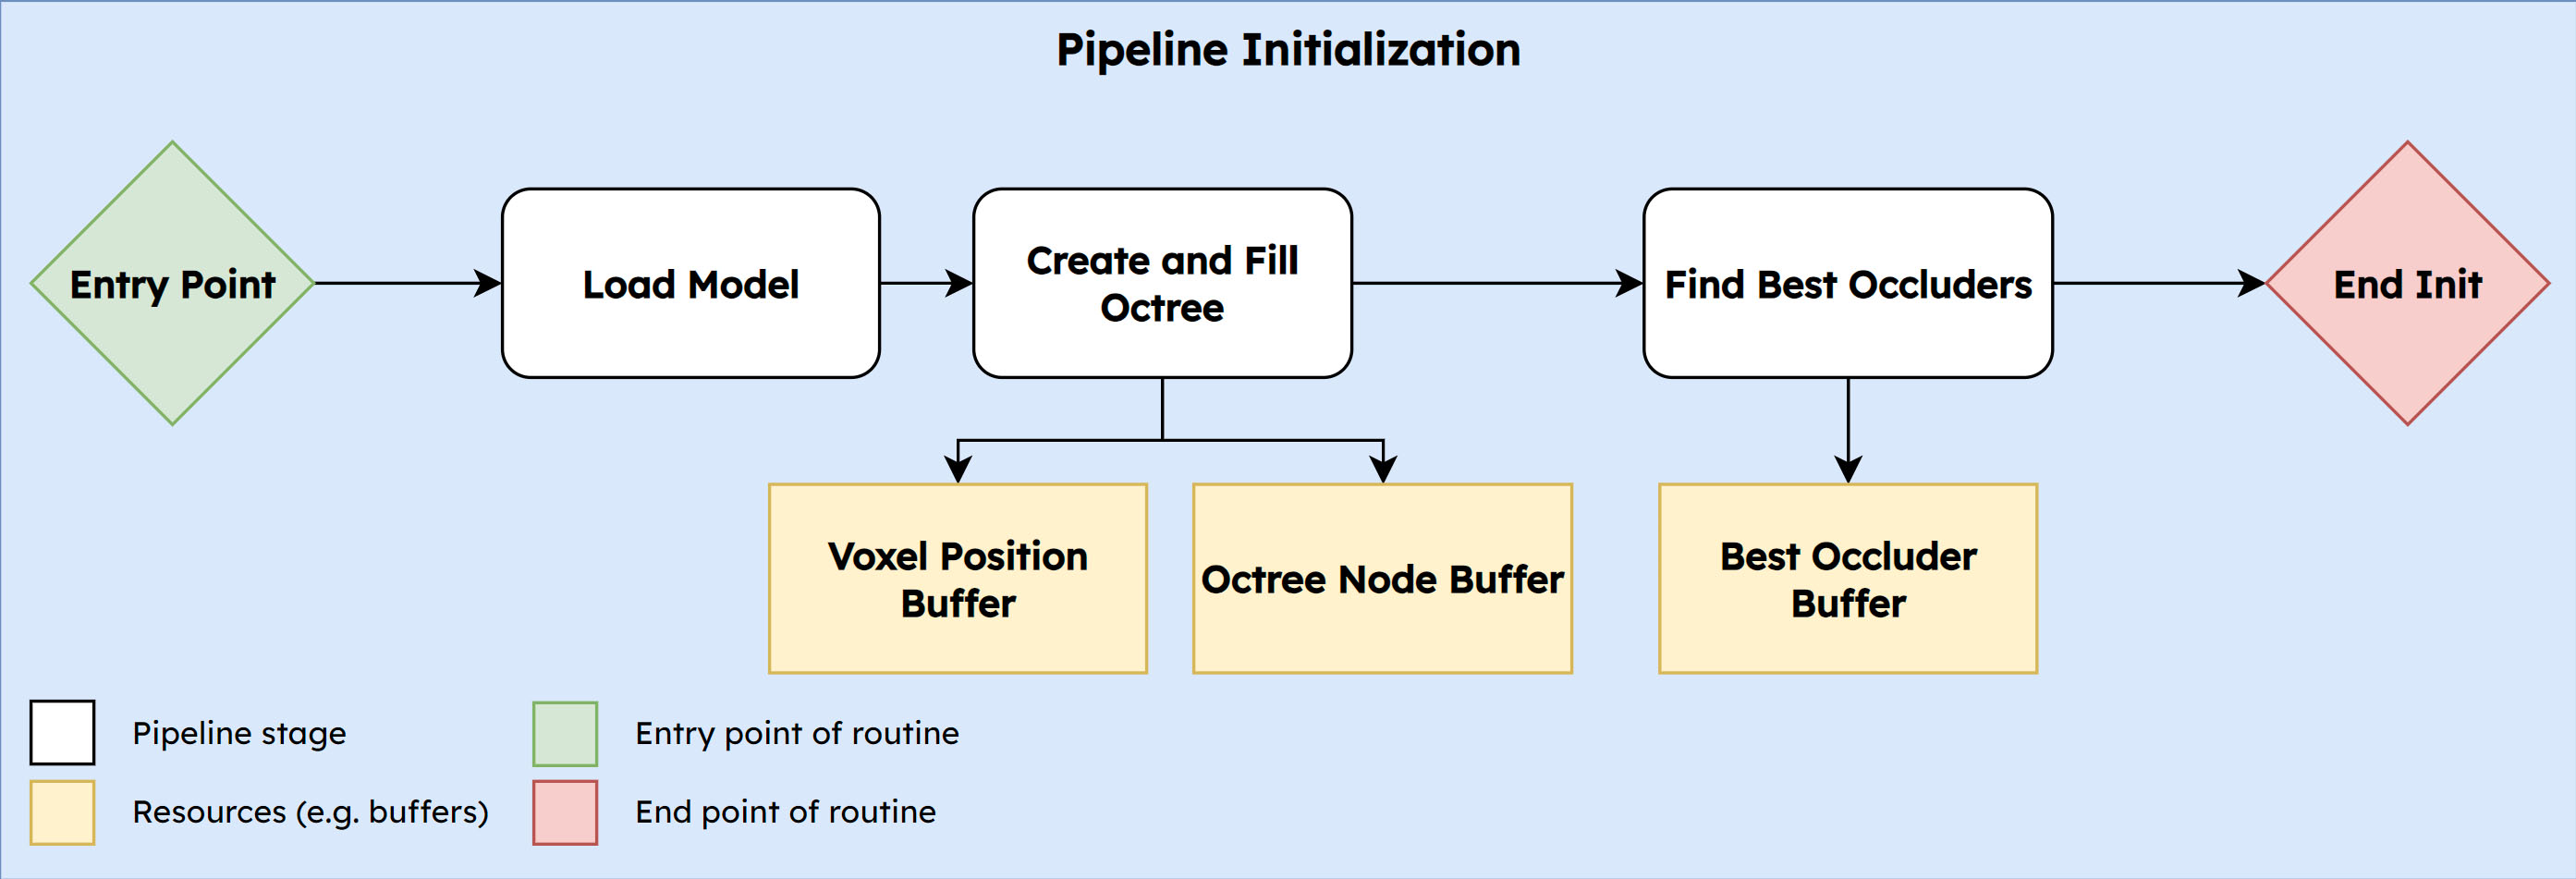
\includegraphics[width=\linewidth]{images/graphics/pipeline-initialization.jpg}
    \caption{The initialization process of the rendering pipeline. Depending on the voxel model, an octree node 
    can hold anything between zero and \emph{n} voxels, \emph{n} being the amount of threads per threadgroup.}
    \label{fig:pipeline-initialization}
\end{figure}

\noindent
The pipeline is split into an initialization routine and an update loop. The initialization is called once during 
the beginning of the execution flow, and the render loop is initiated after the initialization is finished. Then, 
the loop is called each frame. Figure \ref{fig:pipeline-initialization} shows the initialization procedure. 

\subsection*{Voxel Model Loading} \label{subsec-voxel-model-loading}

For the purpose of this experiment, a single, solid voxel mesh is loaded, but this could also be a scene 
consisting of multiple solid voxel models. In the provided implementation, the positions of voxels inside a regular 
grid are loaded, skipping grid cells where no voxels are located. For loading the voxels, the tool \emph{binvox} 
is used \cite{binvox, Nooruddin2003}. It is a command-line tool that converts triangle meshes (e.g. \emph{.obj}) to 
a volumetric voxel representation. The resulting file can be consumed by the engine. Figure 
\ref{fig:trimesh-to-voxel-mesh} shows both the triangle mesh and the processed volumetric voxel mesh. 

\begin{figure}[h]
    \centering
    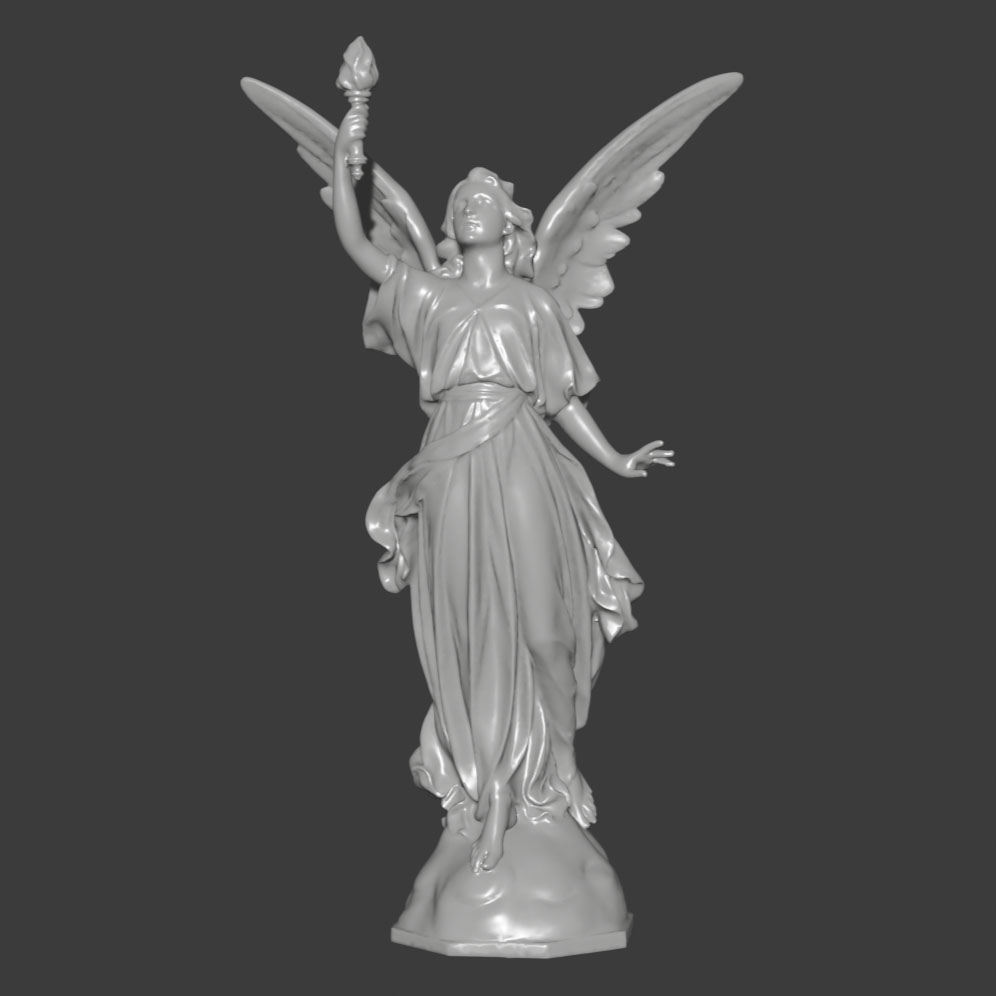
\includegraphics[width=200px]{images/graphics/lucy-triangle-mesh.jpg}
    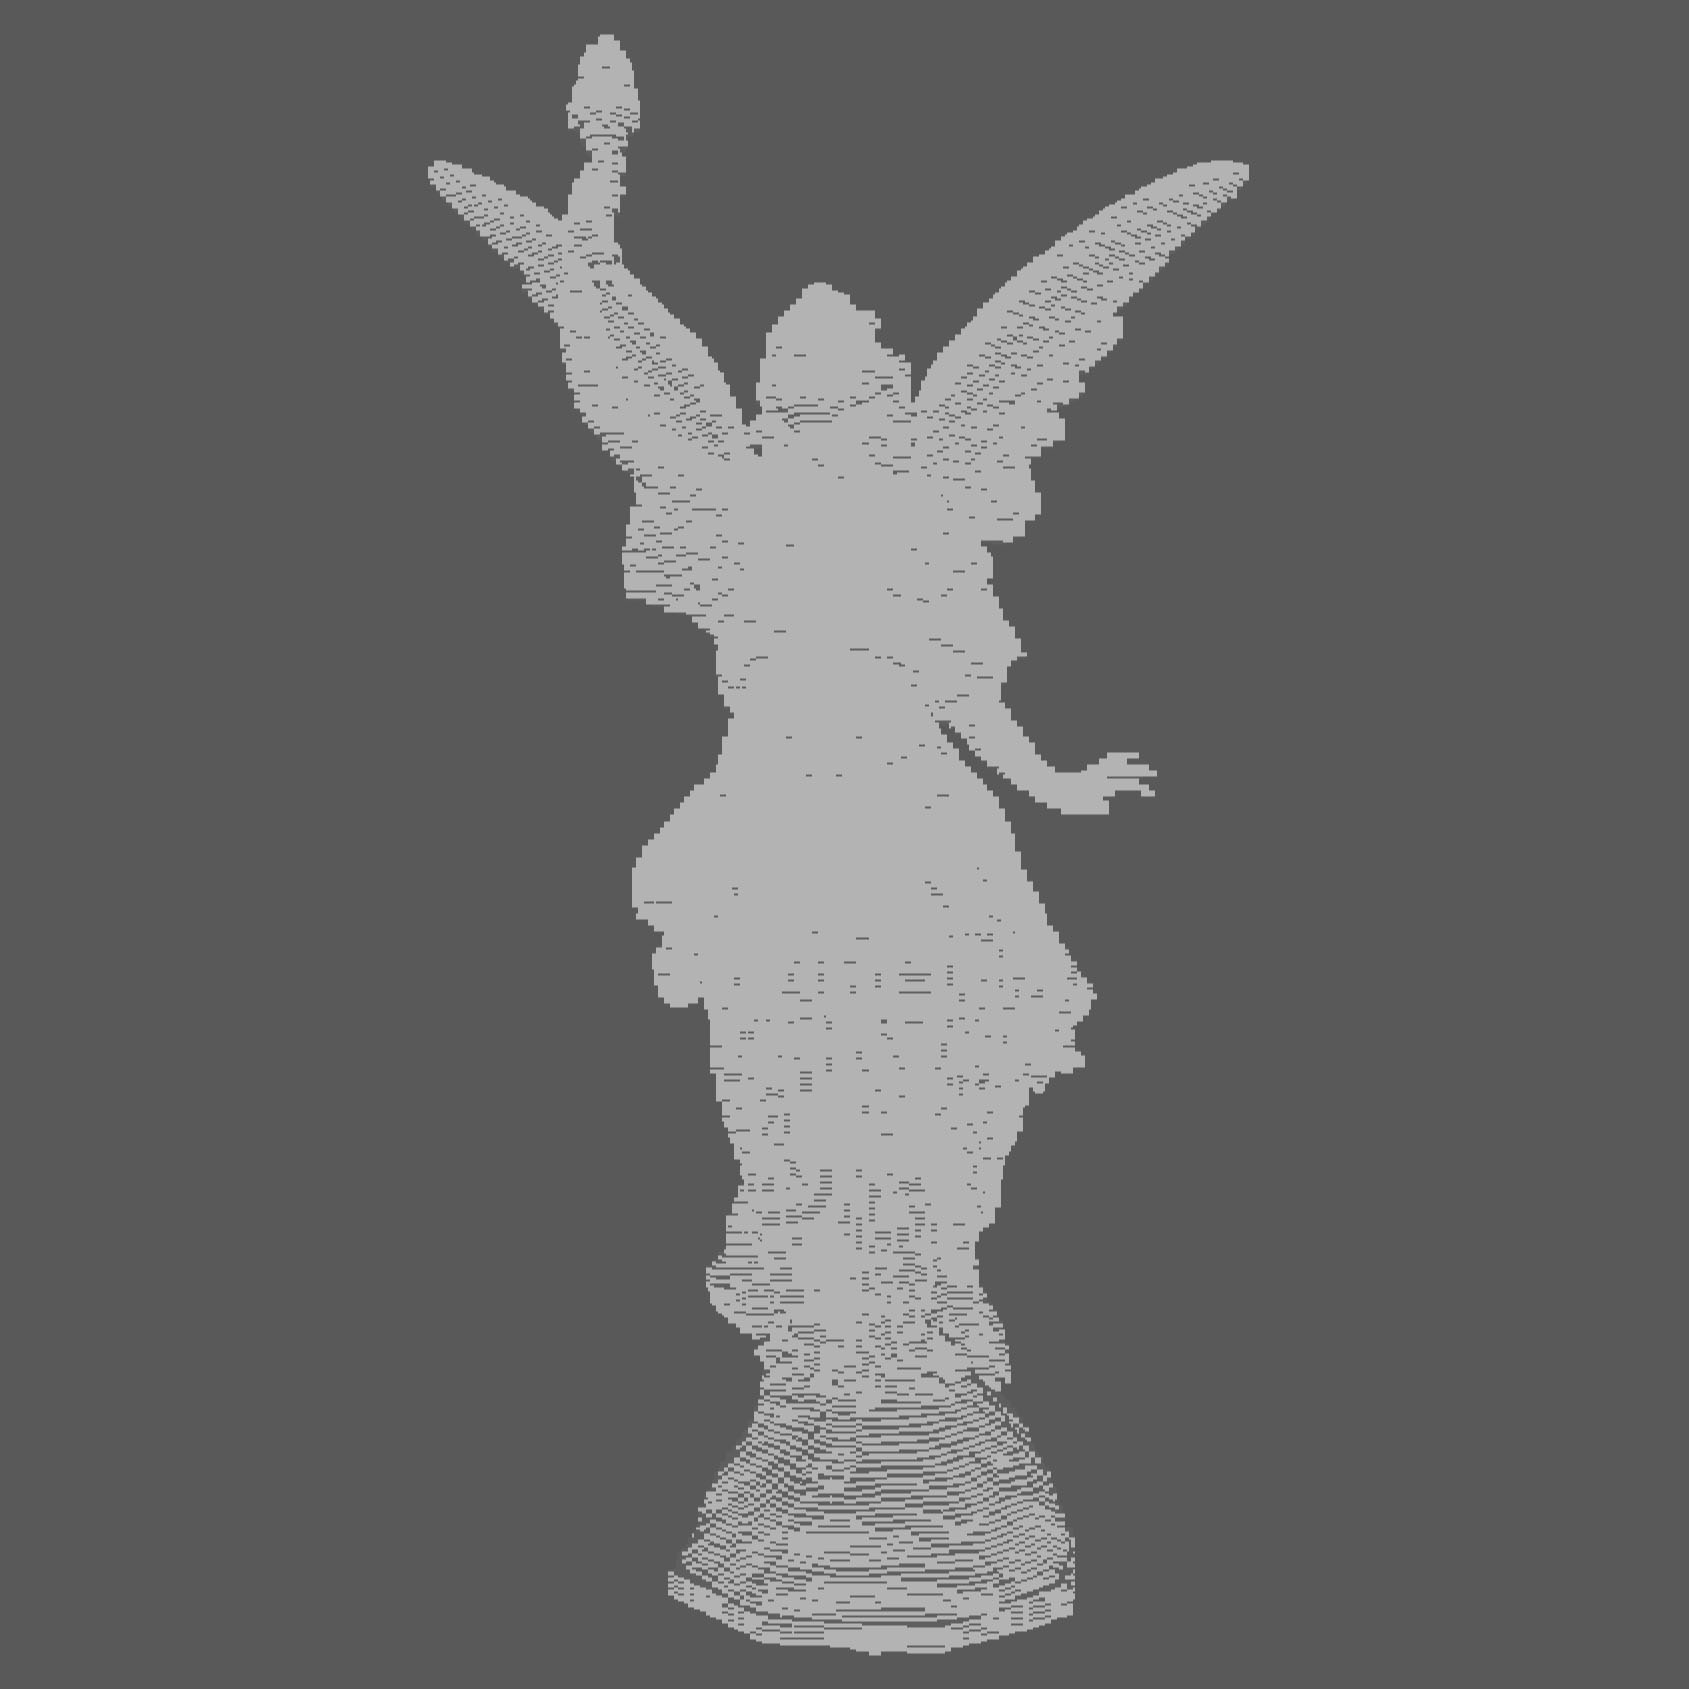
\includegraphics[width=200px]{images/graphics/lucy-voxel-mesh.jpg}
    \caption{The input triangle mesh (left) and the voxelized and parsed voxel mesh (right). 
    Model \emph{Lucy} from \emph{The Stanford 3D Scanning Repository} \cite{Stanford23}.}
    \label{fig:trimesh-to-voxel-mesh}
\end{figure}


\noindent
This model is then processed to fit the requirements of the proposed rendering pipeline. Central to the pipeline 
are the data structures and the \ac{GPU} resources filled with the respective data. To minimize the memory footprint,
the geometry is created on the \ac{GPU}. The only requirement to uniquely identify a voxel then is to know its position.
The main resource is therefore a buffer filled with all the voxel positions as \emph{x, y, z} coordinates. Since \ac{GPU} 
resources usually have to be aligned, 4 bytes of extra space can be used to store the voxel size alongside the position.
It can be used to vary the size of the visible mesh or, for instance, to calculate bounding boxes separately. \\

\noindent
The voxel positions are already sufficient to render the voxel mesh by making each voxel one meshlet. This means that 
individual voxels can be culled based on various meshlet culling techniques outlined in chapter 
\ref{subsec-meshlet-culling}. Each \ac{GPU} thread generates one voxel, or none if the voxel is found to be culled. 
As long as voxels are computed individually, this is very efficient and keeps the memory usage comparably low. But for 
more sophisticated computations, more data is necessary in order to compute spatial characteristics for the voxels. \\

\noindent
Especially when dealing with a lot of voxels, it can be beneficial to cull groups of voxels. So for the proposed 
implementation, it serves well to manage an octree alongside the voxel position data. This additional data structure 
can be used to interpret the data differently. Now each \ac{GPU} threadgroup computes the voxels of one octree node, 
with the maximum amount of voxels per node being equal to the number of threads per threadgroup. Using this layout, 
each thread in a threadgroup again takes care of at most one voxel. The octree node structure can now store additional 
information that can be used for octree node-based culling.

\subsection*{Octree Creation} \label{subsec-octree-creation}

\begin{figure}[h]
    \centering
    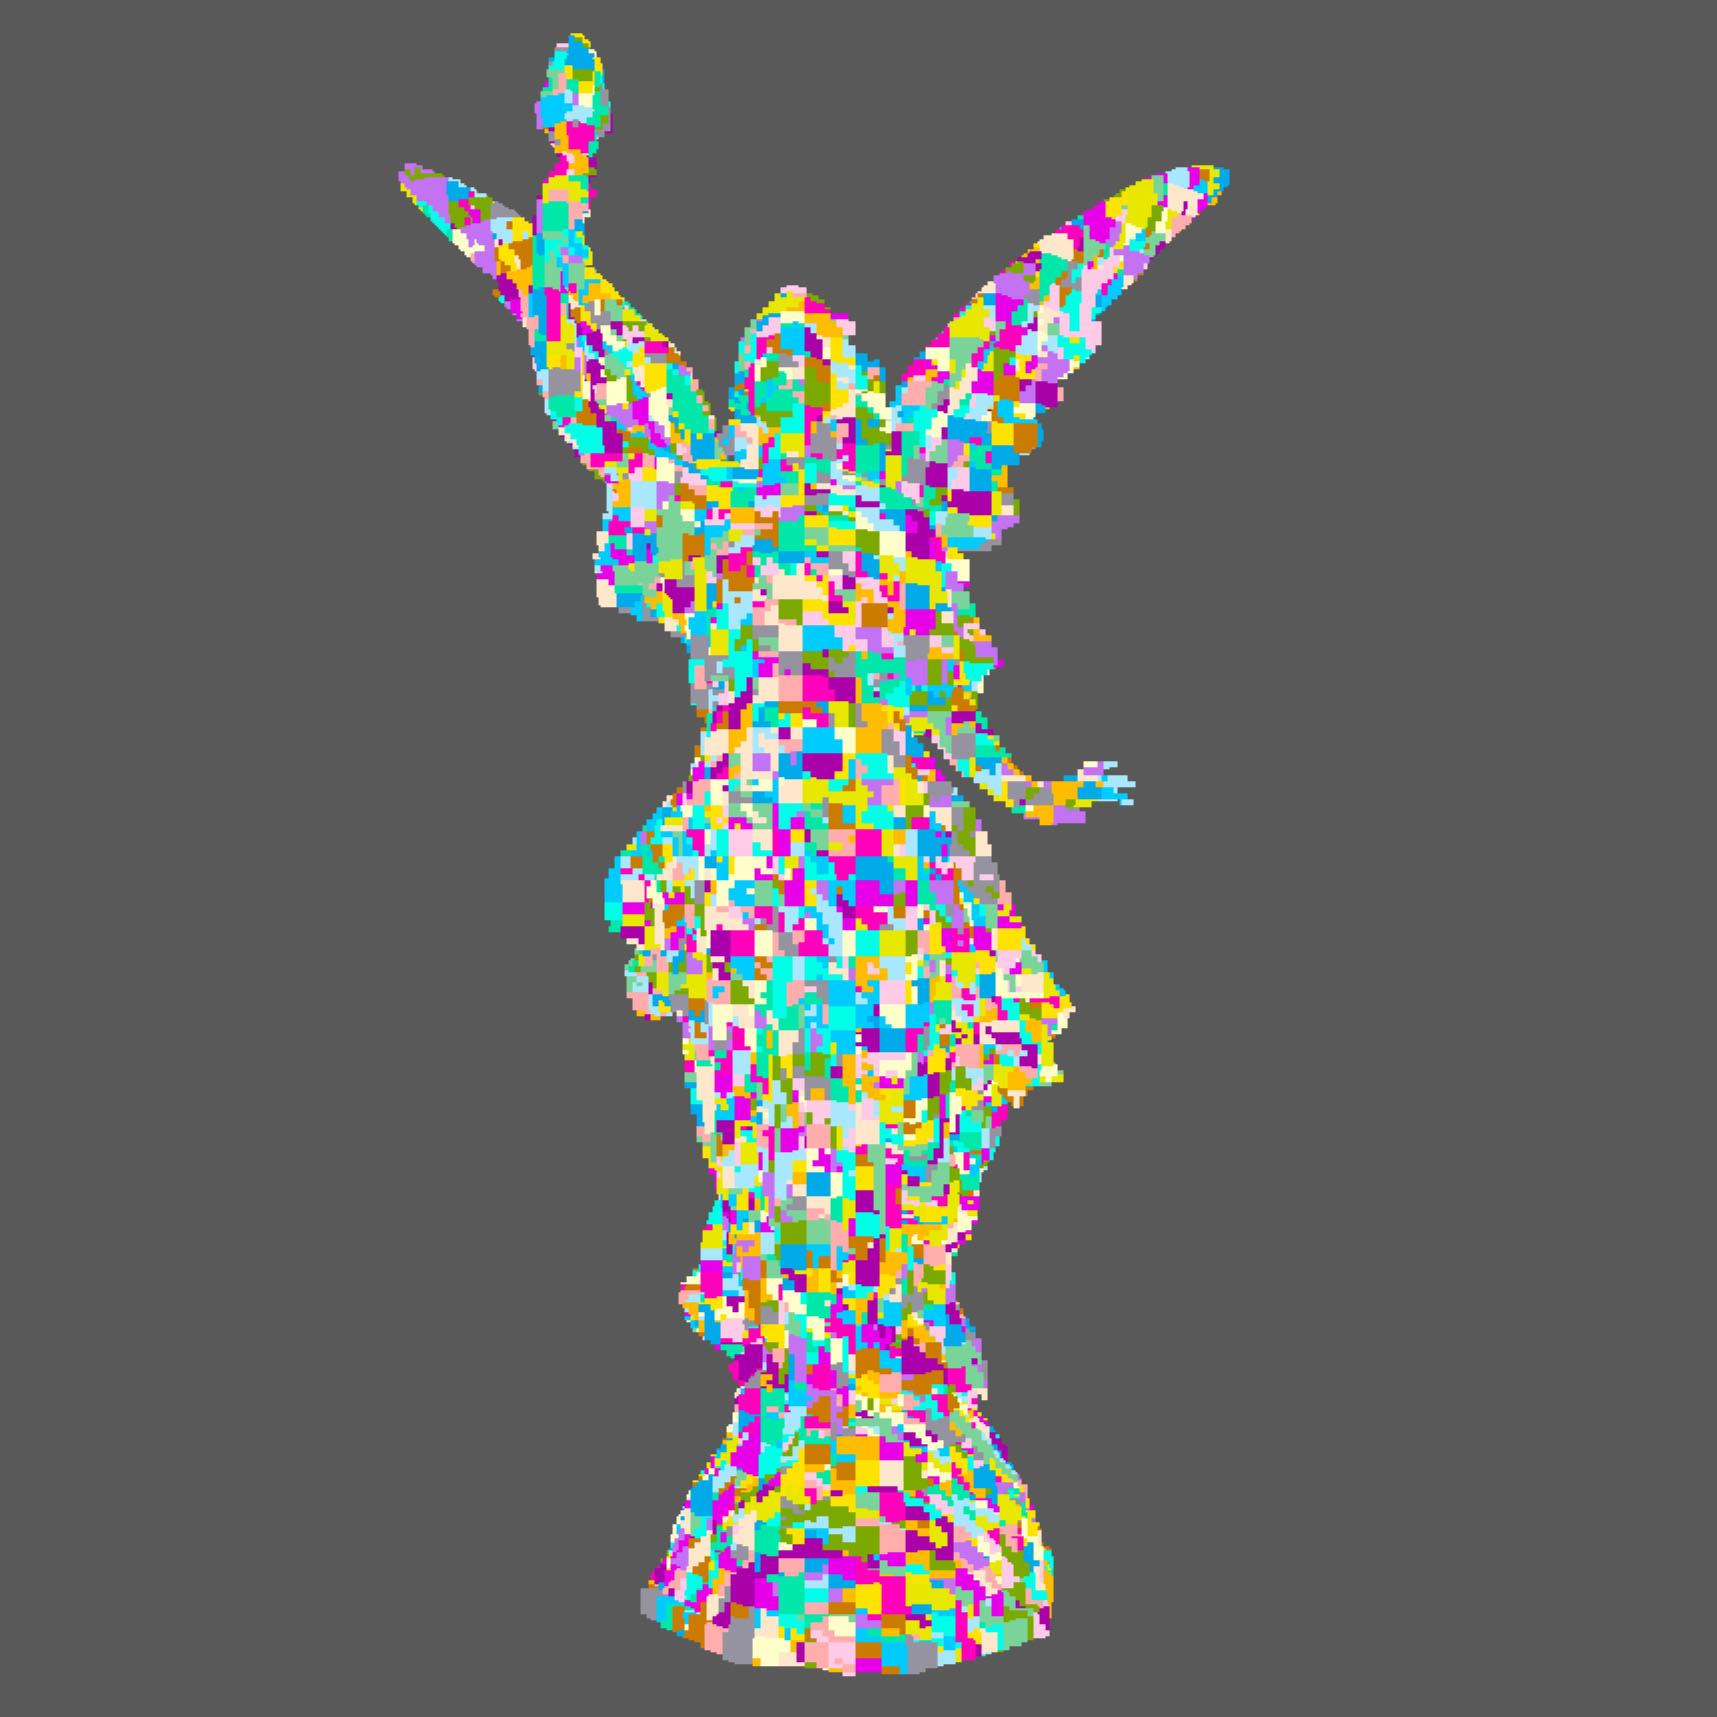
\includegraphics[width=151.5px]{images/graphics/lucy-voxel-octree-viz.jpg}
    
\includegraphics[width=250px]{images/graphics/lucy-voxel-octree-viz-2.jpg}
    \caption{The octree structure visualized. Each color represents one octree node. The whole model contains 
    \emph{470.355} voxels and \emph{19.823} octree nodes, with one leaf octree node holding up to \begin{math} 4 \times 4 \times 4 \end{math}
    voxels.}
    \label{fig:voxel-octree-viz}
\end{figure}

\noindent
After loading any voxel model, an octree is created that covers the entire scene - in the simplest case, there is 
only one model present, so the octree's bounding volume is considered to be equal to the bouding volume of the voxel 
model. As discussed in Chapter \ref{subsec-highres-svo-dags}, it is recommended to use a highly efficient and 
compressed octree implementation like an \ac{SVO} or a Sparse Voxel \ac{DAG} \cite{Kampe2013}. For the purpose of 
this work, a custom octree implementation is used, which refers to indices in the \emph{voxel position buffer}, 
as shown in Figure \ref{fig:voxelpos-octreenode-buffer}. \\

\begin{figure}[h]
    \centering
    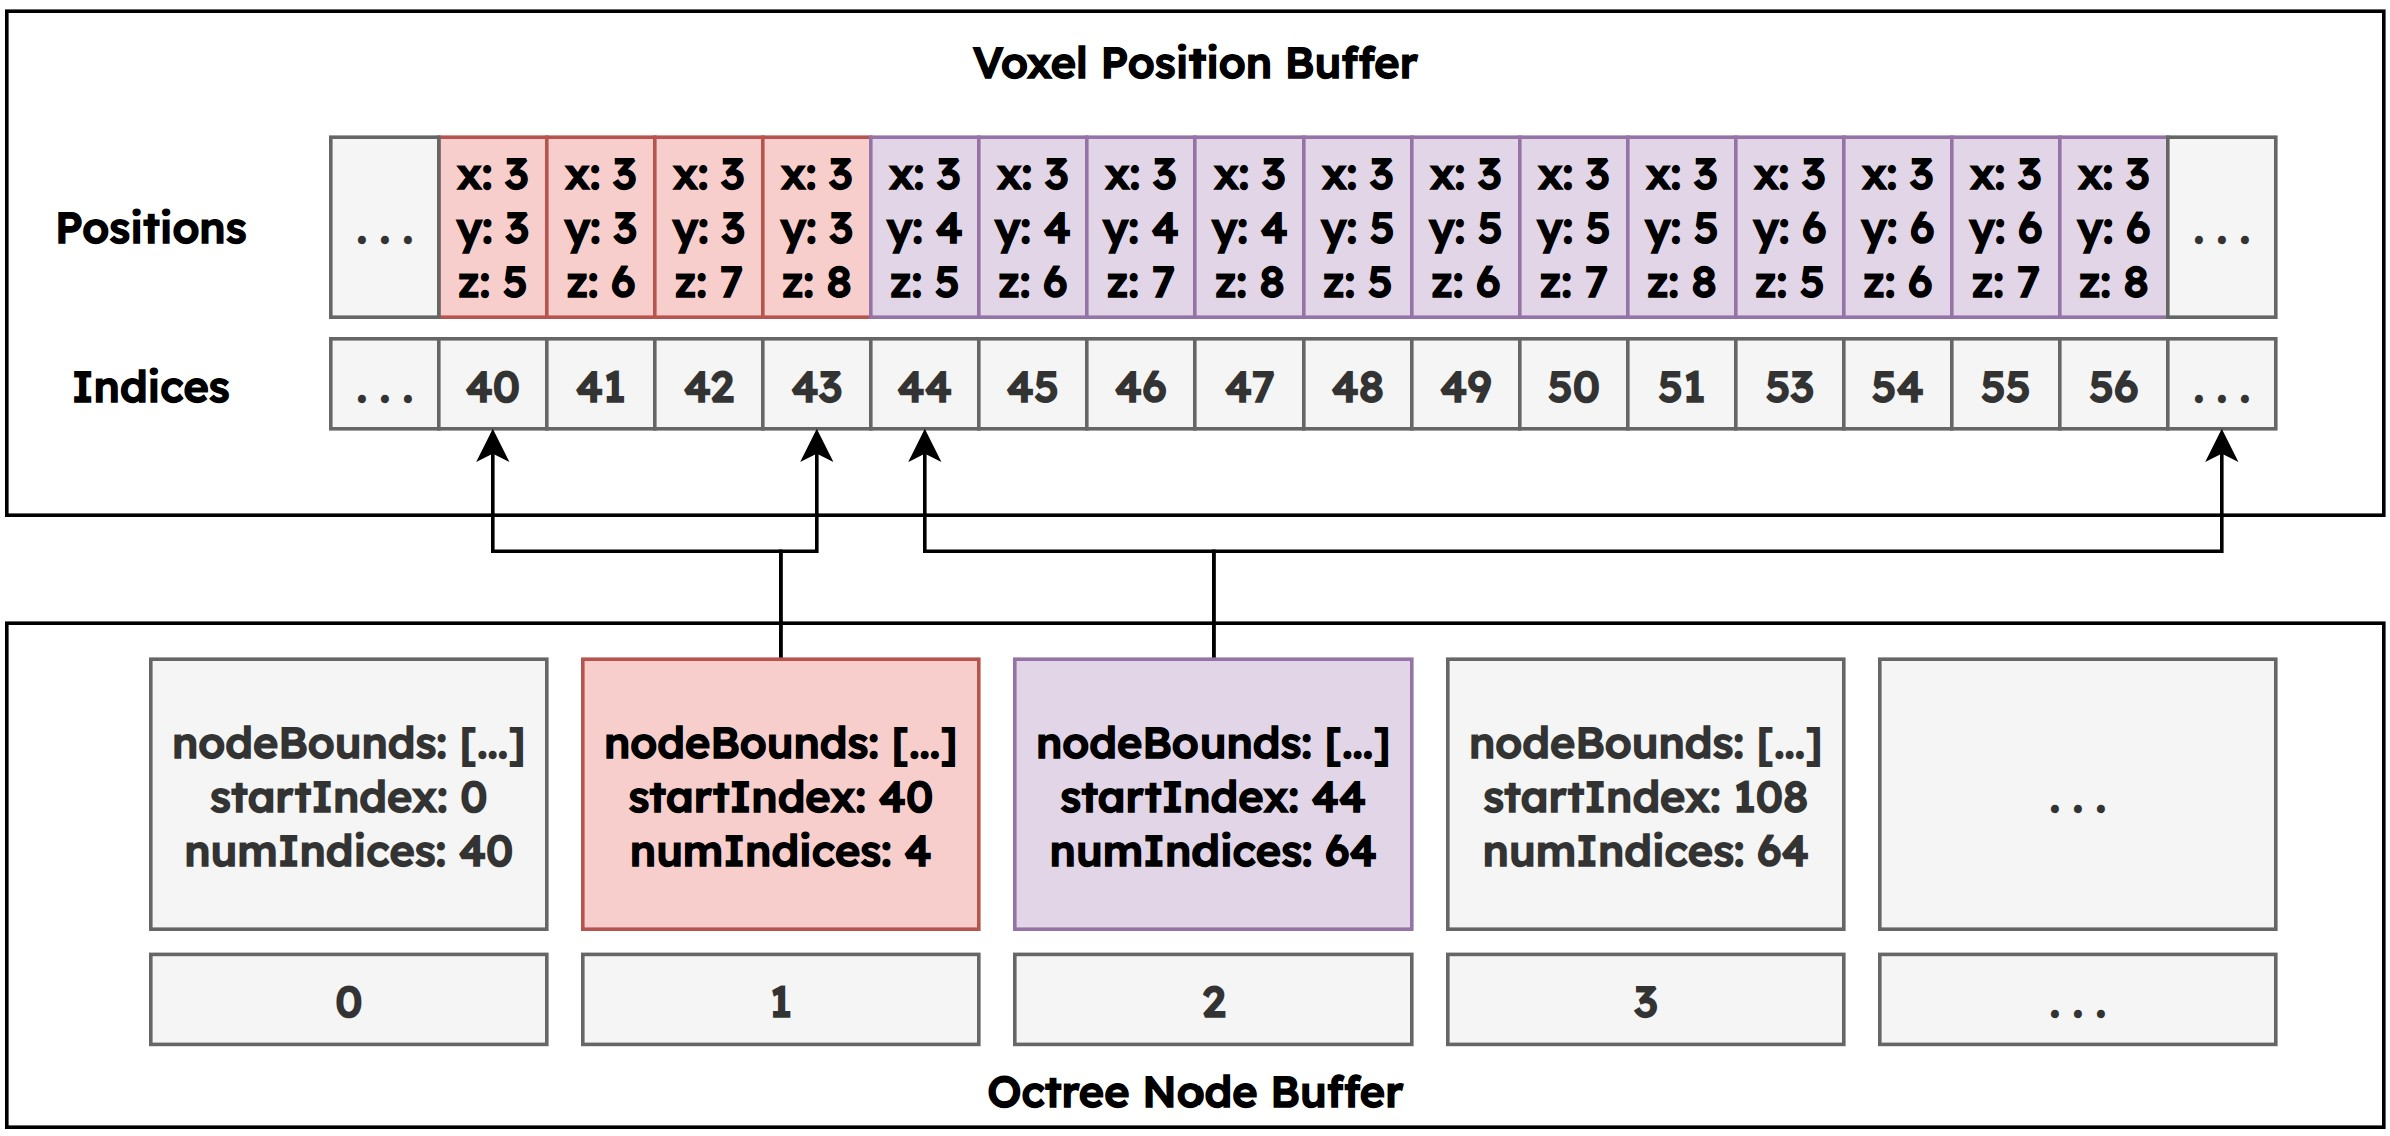
\includegraphics[width=\linewidth]{images/graphics/voxelpos-octreenode-buffer.jpg}
    \caption{The voxel position buffer and the octree node buffer. The latter one providing a 
    specific structure to the first one.}
    \label{fig:voxelpos-octreenode-buffer}
\end{figure}

\noindent
Figure \ref{fig:voxelpos-octreenode-buffer} shows the relation between the octree resource and the \emph{voxel position buffer}.
Since an octree is an inherently hierarchical data structure, it needs to be "flattened" in order to be efficiently fed 
to the \ac{GPU}. This process involves sorting the \emph{voxel position buffer} so voxels within one octree node can be 
located adjacent to one another. The additional "flat" \emph{octree node buffer} then only needs a \emph{start index} 
and a \emph{voxel count} to represent the octree node. Additionally, the octree node's bounds are stored alongside the 
\emph{start index} and the \emph{voxel count}, so octree node-based computations can be executed on the \ac{GPU} side. \\

\noindent
Figure \ref{fig:voxel-octree-viz} shows that the voxels are grouped into octree nodes, which are visualized by distinct 
random colors. 


\subsection*{Best Occluder Selection} \label{subsec-best-occluder-selection}

The next step in the initialization procedure is to precompute the best occluders. As mentioned in chapter 
\ref{subsubsec-two-pass-occlusion-culling}, the best occluders are traditionally authored by artists during the creation 
of the scene. This process is only possible if the models are static in the sense that they do not change in size or 
shape. Although a change in position or rotation is not technically a problem, best occluders are usually inherently 
static. Changes to the properties of the occluder could result in inefficient occlusion queries or even the elimination 
of occluders altogether. \\

\noindent
In the context of volumetric scene representations, this can be a problem since voxel models are often a target of 
manipulation by players or physical interactions. So a predetermination of the best occluders is not possible in the 
way it is for static models. This specific scenario is what the presented approach aims for and why the next step in 
the pipeline preprocesses best occluders. \\

\noindent
Note that this implementation does not include an update of the best occluders. It only serves as an experiment of 
the occlusion culling algorithm in the context of voxel rendering. Updating the best occluders when the voxel model 
is altered needs to be evaluated separately, but is considered to be viable for occasional changes to the mesh. A 
more demanding change to the octree content is given when computing physical interactions within the duration of a 
frame. In this case, further tests need to be done to evaluate the impact on performance. \\

\noindent
The provided approach makes use of the inner, non-visible voxels and approximates them using the octree. For this 
to work, full octree nodes are used as occluders. This means an octree node is a best occluder if the number of 
voxels present within the respective node is equal to the maximum number of voxels possible in that node. Only full 
nodes can be considered best occluders because their shape can be approximated. If the node is not completely filled 
or has holes in it, the approximation will not work. This property of a best occluder is propagated up the tree, as 
long as all eight child nodes satisfy the requirements of being a best occluder. Figure 
\ref{fig:octreenode-filled-non-filled} shows three possible leaf nodes. 

\begin{figure}[h]
    \centering
    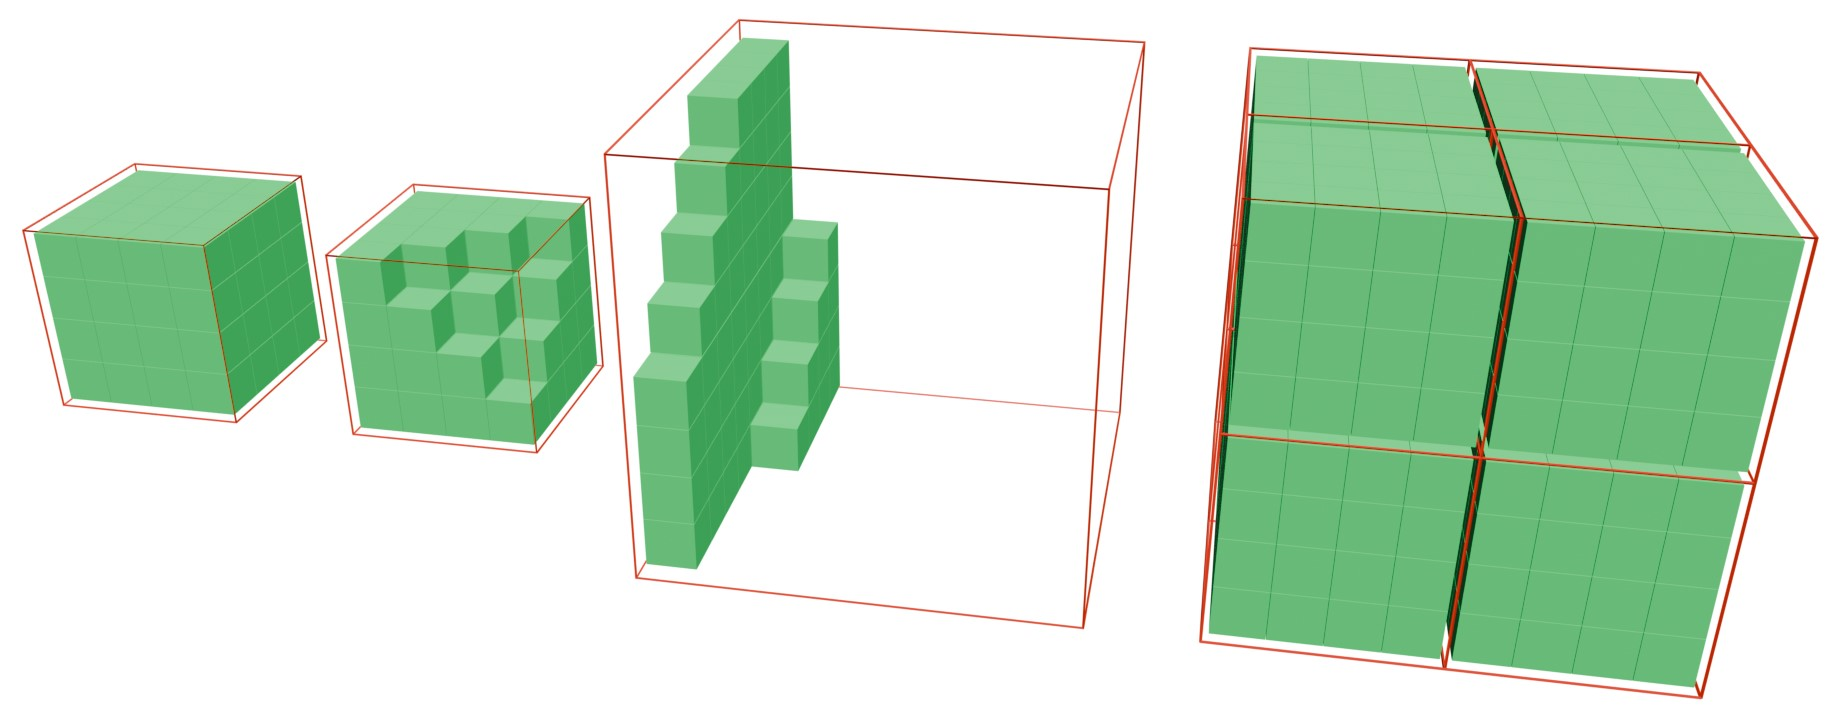
\includegraphics[width=300px]{images/graphics/octree-nodes-filled.jpg}
    \caption{Four possible \emph{octree leaf node} setups. The left most node is completely filled up to its 
    boundaries and therefore considered to be a best occluder. The middle left node is not completely filled 
    and therefore not considered to be a best occluder. The middle right node has larger boundaries but can 
    still be a leaf node as long as the amount of voxels in the node doesn't force the node to split. Since 
    it is not completely filled it is not considered to be a best occluder. The right node has eight full child 
    nodes and is therefore considered full and a best occluder. The gaps between voxels and the node boundaries 
    are only for visualization purposes.}
    \label{fig:octreenode-filled-non-filled}
\end{figure}

\noindent
During the depth prepass, the best occluders are drawn as "large voxels", which are the size of the respective 
best occluder node. This can be achieved by simply reusing the mesh shader used in the normal draw call and 
inputting the node's position and bounds. This way, a whole node gets drawn instead of the individual voxels, 
reducing the computation cost for drawing the best occluders considerably. The best occluders are stored in a 
separate buffer so they can be dispatched efficiently. \\

\noindent
This concludes the initialization of the pipeline. When changes are applied to the voxel data, the voxel buffer,
the octree node buffer, and the best occluder buffer need to be updated accordingly. Alternatively, the best 
occluders can be implicitly calculated on the basis of the octree node buffer. This would make the best 
occluder buffer redundant but would result in a higher dispatch count with a lot of discarded nodes, 
where the criteria for best occluder are not met. Since all computations are more or less in parallel, this 
will not affect frametimes for a moderate amount of octree nodes. Nevertheless, since only static voxel models with 
no runtime alternation are assumed for this work, a static, pre-calculated buffer for best occluders can be used.


\section{Rendering Loop} \label{sec-rendering-loop}

\begin{figure}[h]
    \centering
    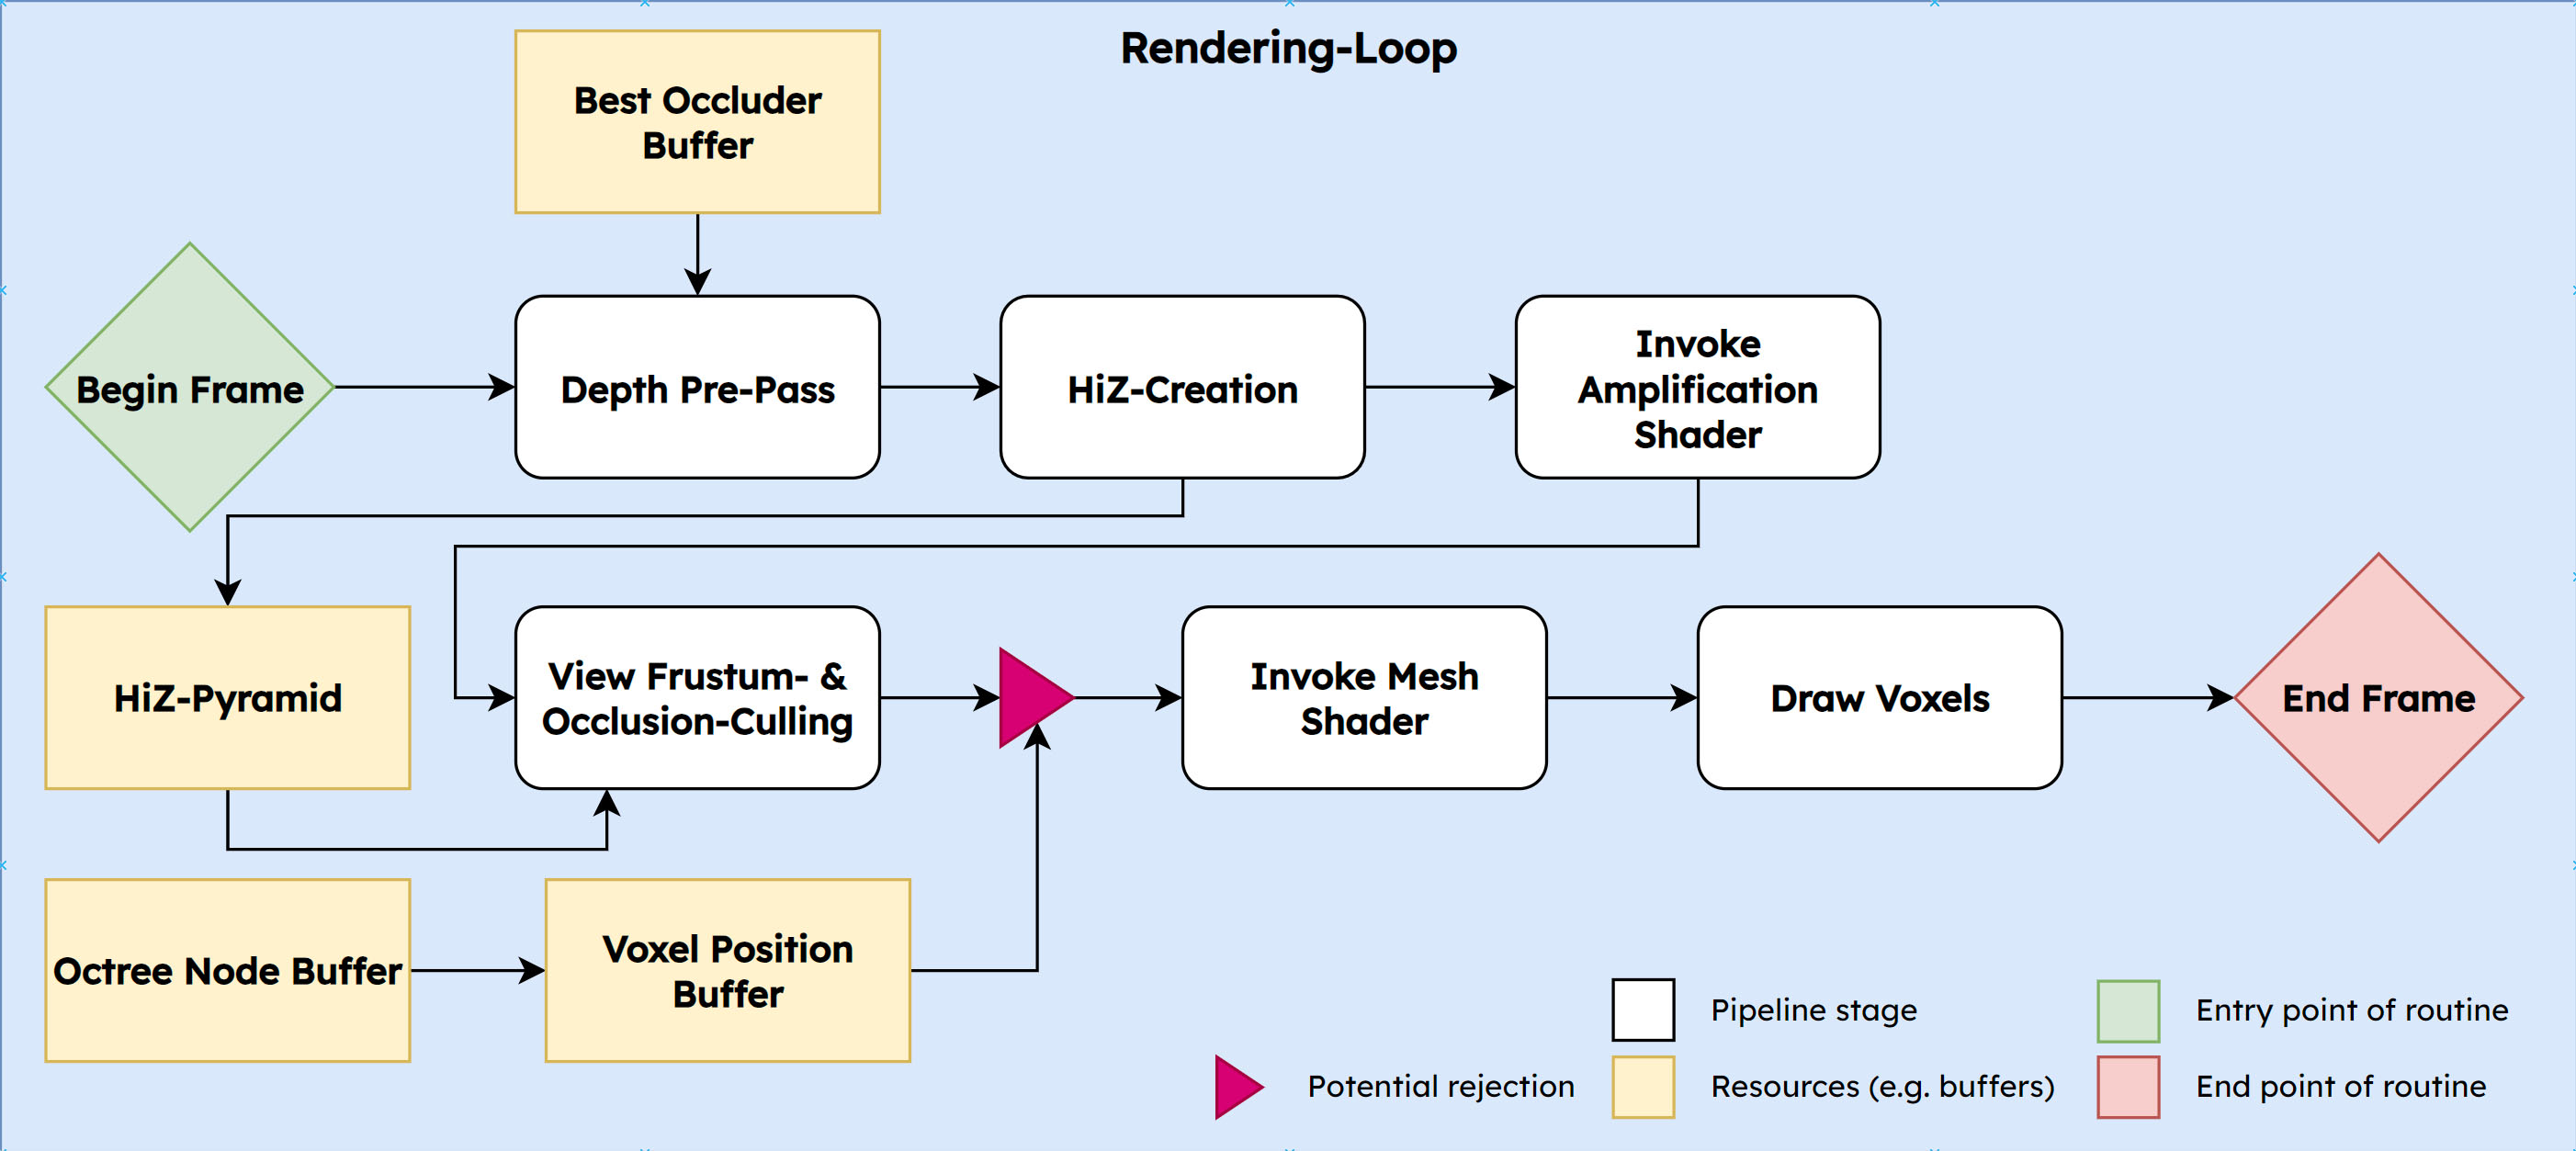
\includegraphics[width=\linewidth]{images/graphics/rendering-loop.jpg}
    \caption{The rendering loop of the rendering pipeline. The red sub-stage of the render loop marks the dispatch 
    of the meshlets, involving the voxel positions and the octree node data. If an octree node or voxel is considered 
    to be culled, the loop ends with the task shader.}
    \label{fig:pipeline-loop}
\end{figure}

\noindent
The rendering loop consists of three main steps: The depth prepass including \ac{HiZ} generation, the 
task shader, and the mesh shader. The different stages consume and generate various data buffers 
and textures, as shown in Figure \ref{fig:pipeline-loop}. 

\subsection*{Depth Pre-Pass} \label{subsec-depth-prepass}

The frame computation starts with the depth prepass, which is the custom render pass central to the 
occlusion culling. In this pass, a compute shader is invoked that takes the best occluders and draws 
them to the depth buffer. This depth pass does not draw to the back buffer, making the computation 
relatively efficient. To get a better understanding of what this means, Figure \ref{fig:best-occluder-viz} 
shows the best occluders. Note that the best occluders in this visualization are not hierarchically 
aggregated, which results in a slightly different visual result than what the actual depth buffer shows. 

\begin{figure}[h]
    \centering
    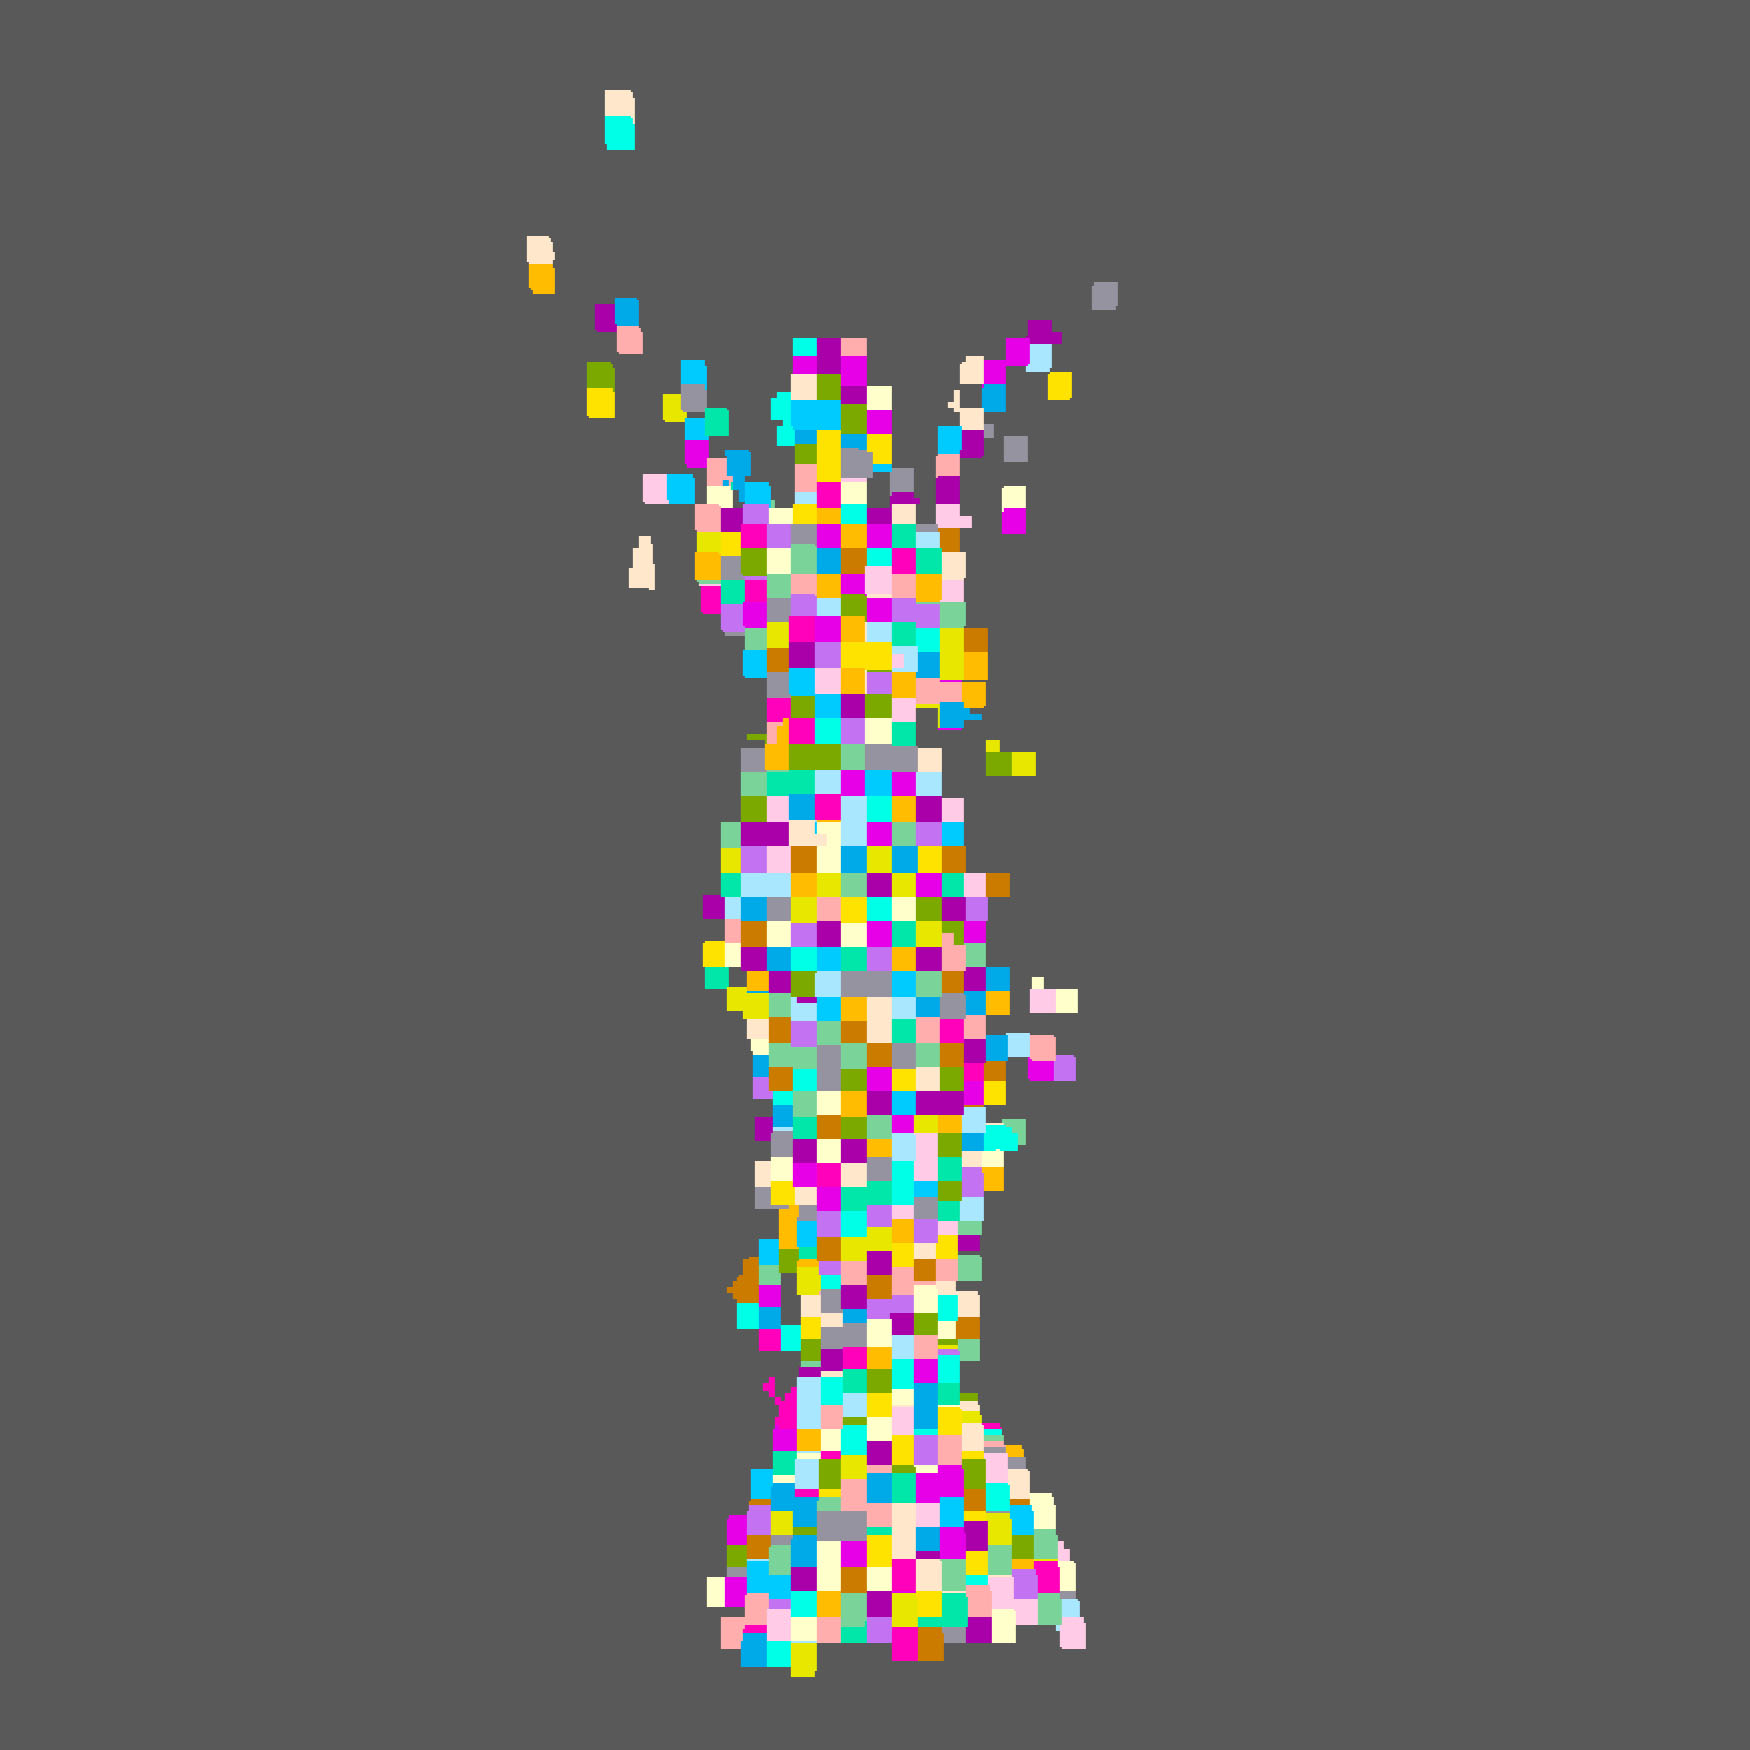
\includegraphics[width=200px]{images/graphics/lucy-best-occluders-viz.jpg}
    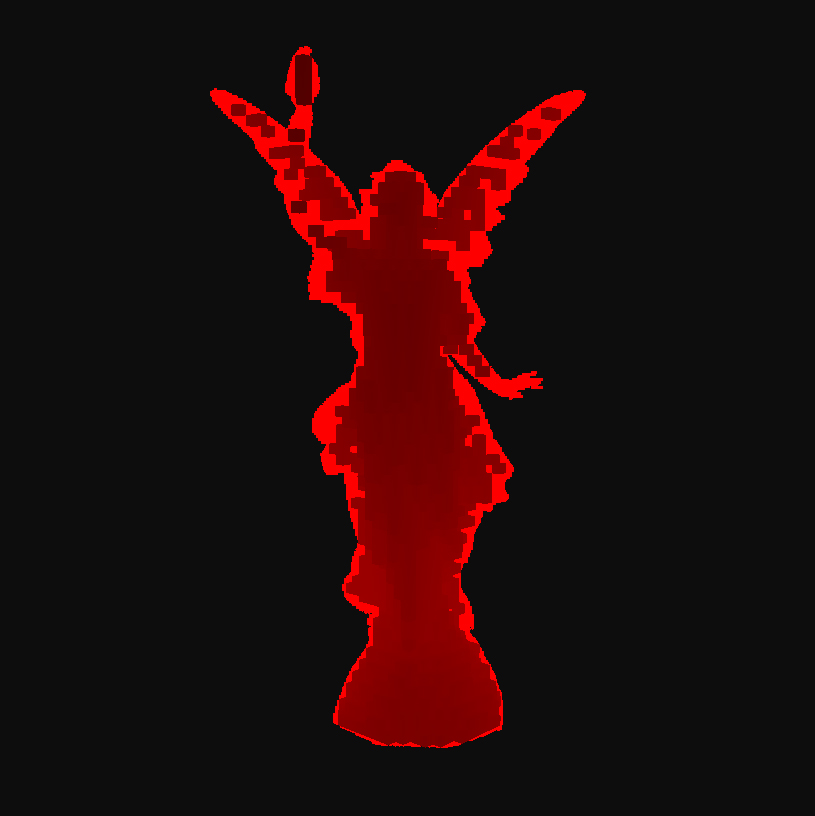
\includegraphics[width=200px]{images/graphics/lucy-best-occluders-diff-viz.jpg}
    \caption{A visualization of the best occluders (left) and the best occluders blended with a silhouette 
    of the whole voxel model (right). Each color represents one octree node which is considered to be a best occluder.
    The best occluders describe the non-visible core of the model and can be aggregated and used to occlude 
    many non-visible voxels during rendering.}
    \label{fig:best-occluder-viz}
\end{figure}


\subsection*{HiZ Generation} \label{subsec-highz-generation}

\begin{figure}[!htb]
    \centering
    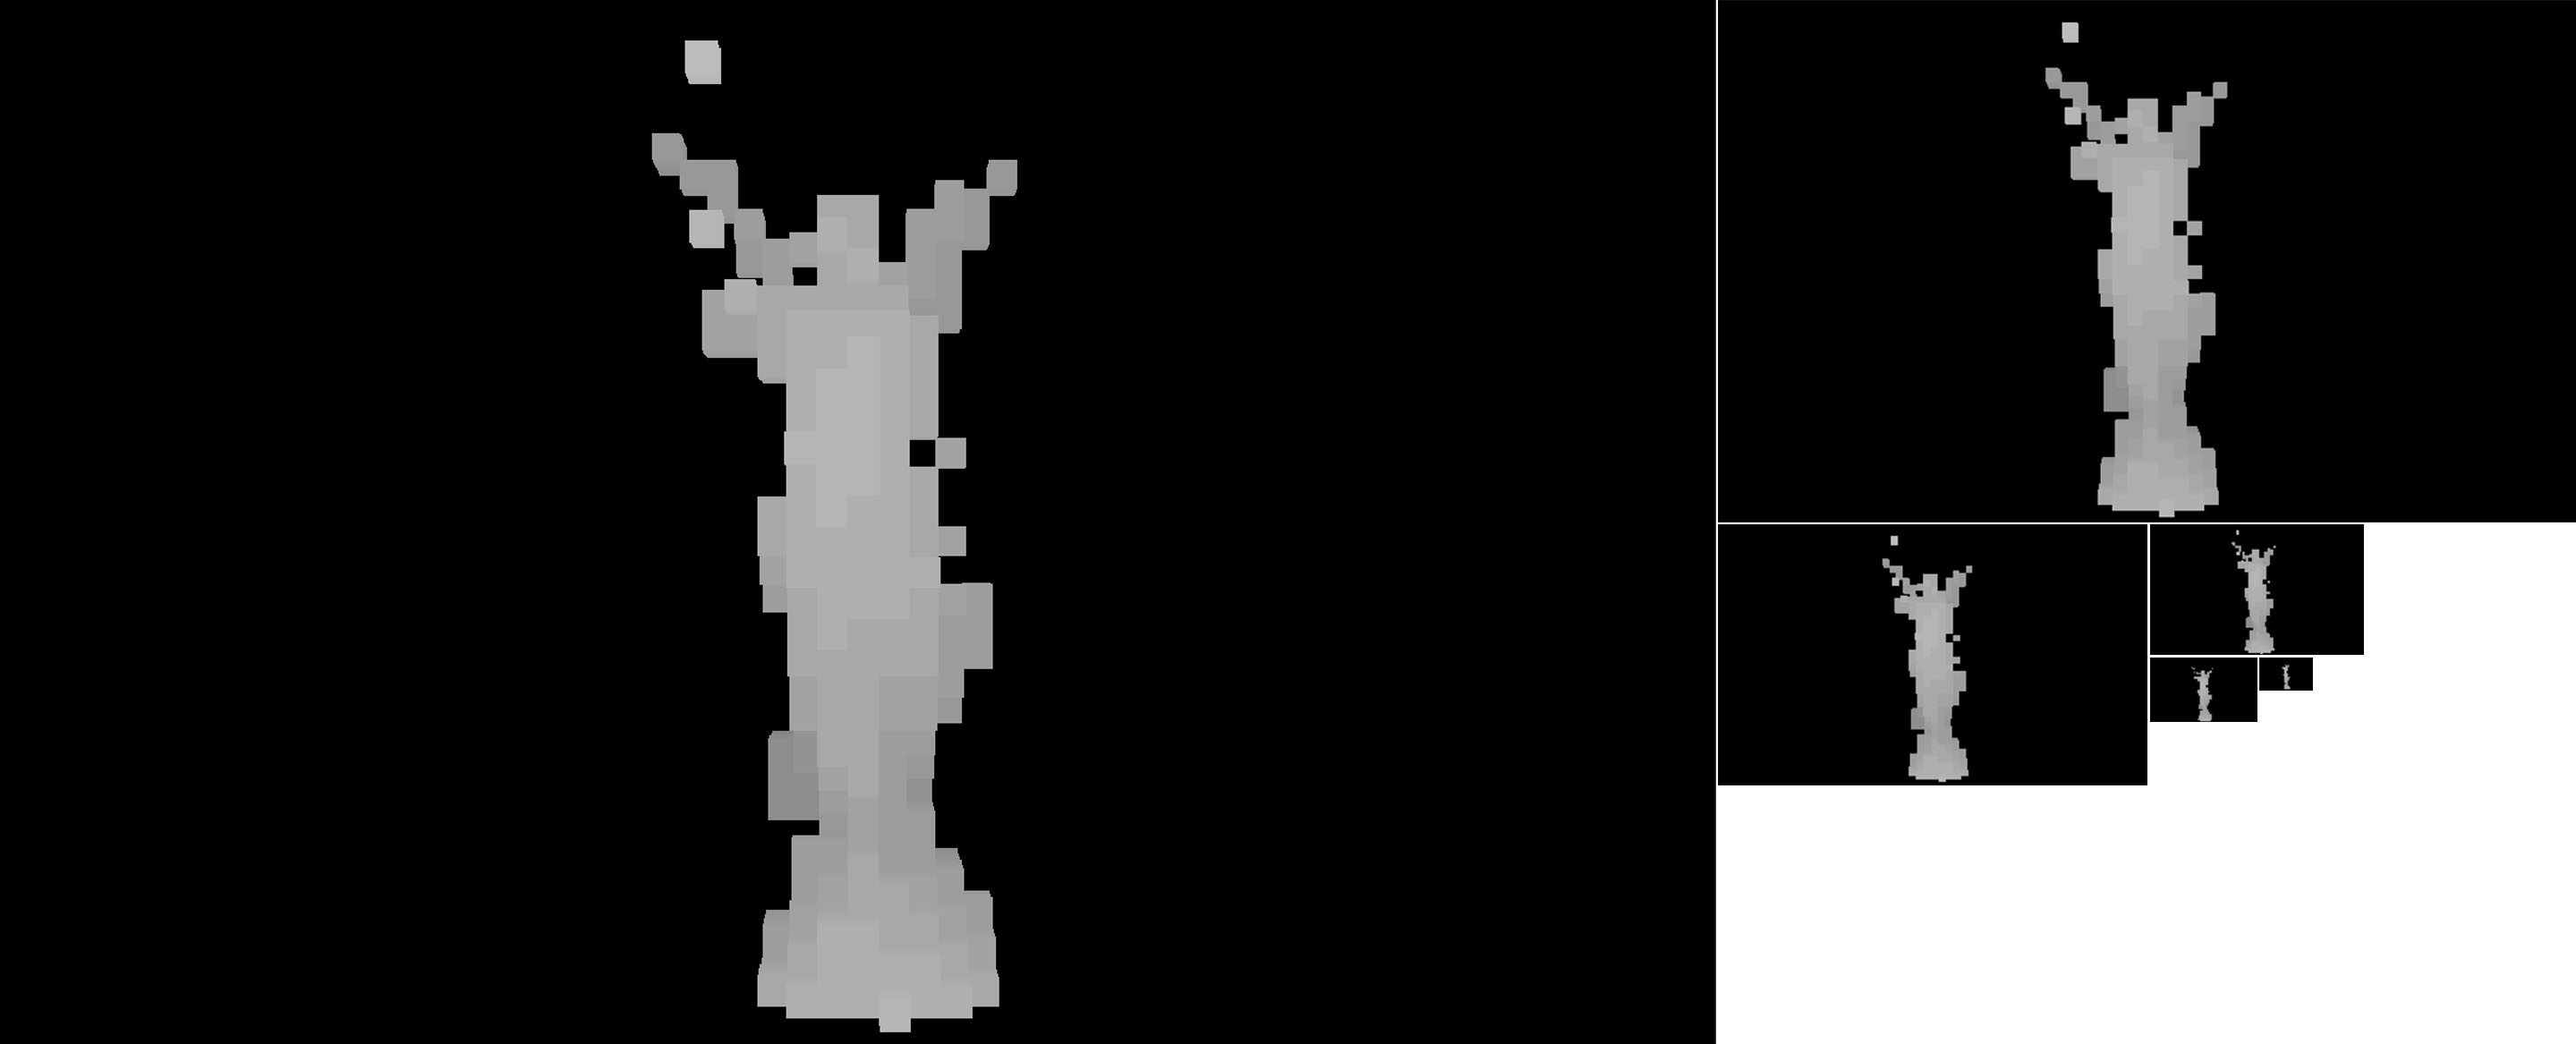
\includegraphics[width=\linewidth]{images/graphics/lucy-hiz-pyramid-inverted.jpg}
    \caption{The \ac{HiZ} pyramid featuring the full resolution depth buffer as well as the individual mip map 
    levels. The color representation was inverted for better visualization.}
    \label{fig:lucy-hiz-pyramid}
\end{figure}

\noindent
After drawing the best occluders to the depth buffer, it is copied into the \ac{HiZ} texture resource. Subsequently, 
the \ac{HiZ} pyramid is generated by a compute shader, which samples four texels of the input texture (the full resolution 
depth buffer) and outupts the farthest depth value to the respective higher mip level. After all mip levels are constructed, 
the \ac{HiZ} pyramid can be used for occlusion culling. The final \ac{HiZ} pyramid is illustrated in figure 
\ref{fig:lucy-hiz-pyramid}. In the pipeline diagram in Figure \ref{fig:pipeline-loop}, a part of this chain of mip-maps is shown.


\subsection*{Culling} \label{subsec-task-shader}

When the task shader is invoked, each thread group is operating on one octree node. Before the 
occlusion culling is executed, the camera view frustum culling removes non-visible octree nodes. 
Figure \ref{fig:bunny-frustum-culling} shows a partially frustum-culled model from an outside 
perspective. \\

\begin{figure}[!htb]
    \centering
    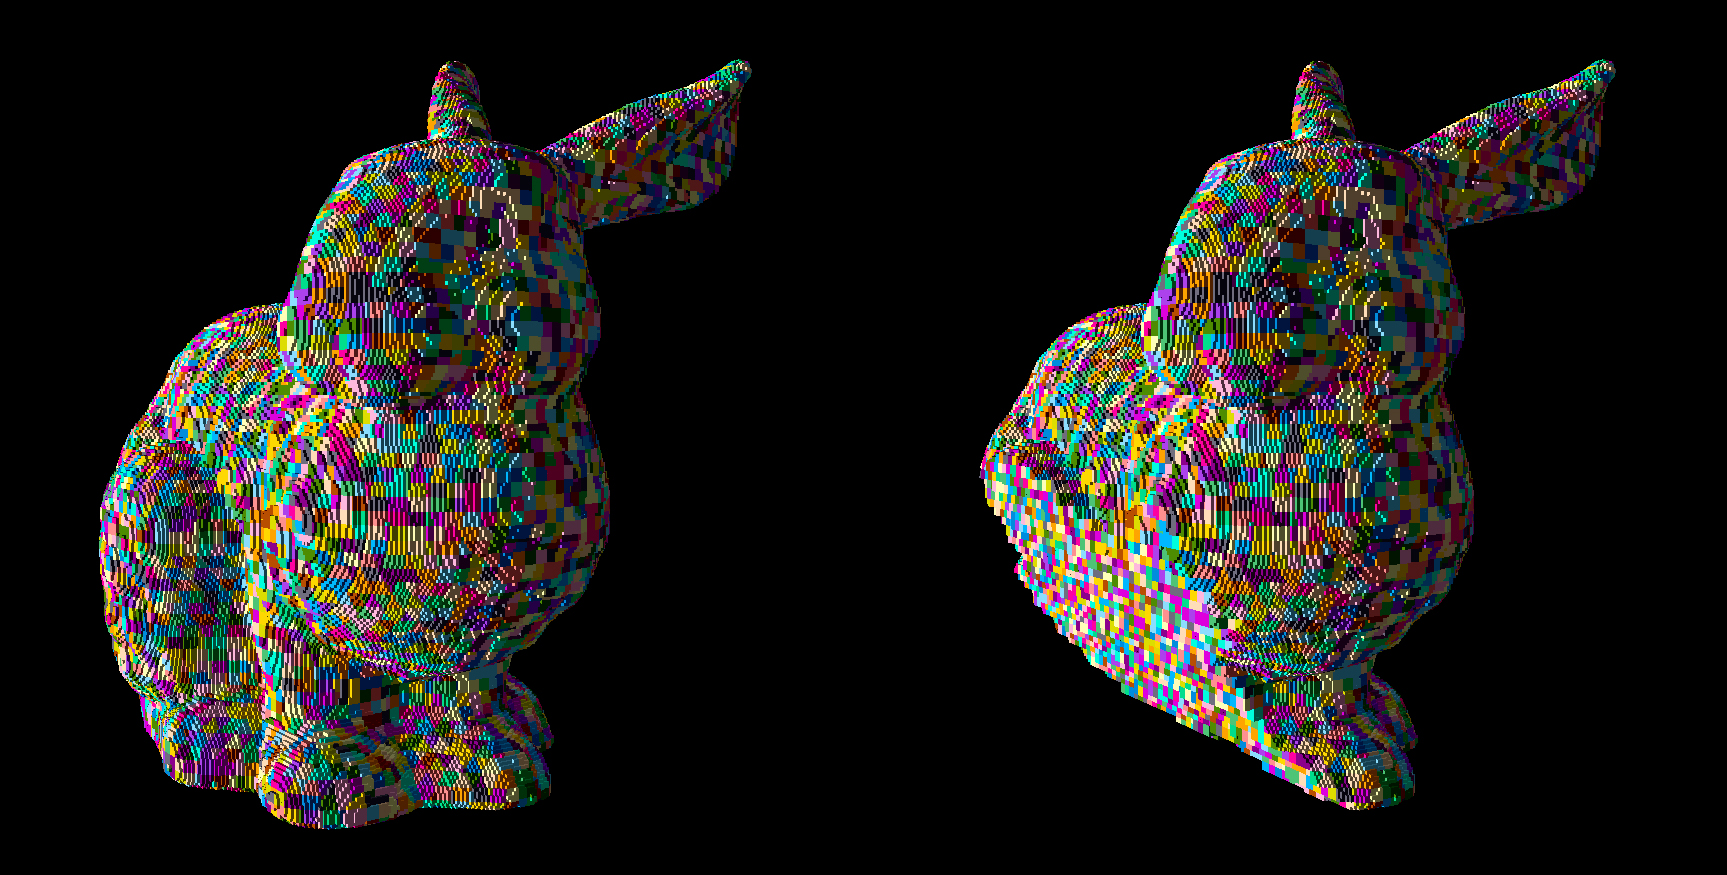
\includegraphics[width=300px]{images/graphics/bunny-frustum-culling.jpg}
    \caption{Left: The whole \emph{Bunny} model without any culling. 
    Right: The whole \emph{Bunny} model culled against the view frustum as seen from an outside perspective. 
    Octree nodes which are not in the view frustum are being culled and are therefore not visible.}
    \label{fig:bunny-frustum-culling}
\end{figure}

\noindent
Nodes that were not culled using the view frustum are then drawn, checking each voxel for occlusion against the 
\ac{HiZ} texture and its mip maps. This operation introduces additional overhead, which is normal for any acceleration structure. 
The goal is always to apply it to a scenario where the additional overhead is compensated by the acceleration it provides. 
In this case, the visible voxels might have to pass the whole \ac{HiZ} structure. The non-visible voxels, however, will likely 
exit early after just a few operations, comparing against the mip map hierarchy. In a volumetric representation, the candidates 
for non-visible voxels are plenty, as usually, only a fraction of the voxel data needs to be drawn at any time. Essentially, 
all voxels, but the outer, visible layer, can be omitted.

\subsection*{Drawing} \label{subsec-mesh-shader}

The mesh shader executes the appropriate transformations, constructs a uniform voxel around the voxel position, 
and outputs the geometry. The voxels in a \ac{GPU}-driven approach can be completely generated on the \ac{GPU}, 
minimizing the memory bandwidth used per frame. This optimization technique is not only efficient but also 
trivial for uniform, static voxel geometry. When dispatching one voxel per thread, one voxel corresponds 
to one meshlet, making pre-computation completely redundant, as opposed to the common precomputation of meshlets, 
as mentioned in Chapter \ref{sec-mesh-shading}. UVs, normals and other geometry data or attributes are 
trivial to determine for uniform voxels and are also looked up in the mesh shader.


\section{Occlusion Culling Algorithm} \label{sec-occlusion}

The occlusion culling algorithm is the central part of the pipeline and thus deserves a more detailed coverage. The 
basic implementation is very similar to the ones provided by Aaltonen et al., Greene et al., or Karis et al. 
\cite{Aaltonen2015,Greene93,Karis2021}. It relies on the pre-computations discussed above and can be applied to the 
octree nodes or to individual meshlets. Usually, octree nodes are culled in this process, as \cite{AkenineMoeller2018}
points out. However, using the mesh shading pipeline, it has become possible to cull more fine granular by using 
meshlet bounding volumes as occludees. One advantage is that geometry can be culled, even when the occluder doesn't 
fully overlap the octree node. Therefore, even small instances in the scene can occlude a lot of geometry, resulting 
in better performance overall. On the other hand, this approach requires a lot more computations because all meshlets 
are checked against the \ac{HiZ} pyramid. It is necessary to make precise measurements in order to find out which 
approach works best under the given circumstances.


\subsection*{Visibility Computation} \label{subsec-visibility-computation}

As mentioned before, the task shader is used to pre-select and pre-process the scheduled geometry data, 
which in this case is just the position of an individual octree node and all the voxels inside of the node. 
This precomputational step is used for visibility checking, i.e., view frustum culling and occlusion culling. 
Since the task shader is based on the compute architecture, this pipeline step is realized using a standard 
compute-like code structure. \\

\noindent
To check for visibility, projected bounding boxes need to be constructed and checked against the 
\ac{HiZ} pyramid. This step can be highly parallelized by using one \ac{GPU} thread per bounding box 
calculation. The first step involves the projection of the bounding box onto the view plane, which results 
in a clip-space representation of the data. This early projection is done for all eight vertices of the 
bouding box, so the \emph{min} and \emph{max} values on each axis can be calculated to end up with clip-space, 
and eventually with screen-space coordinates. The \emph{min} and \emph{max} values for each axis represent 
a screen-space rectangle, which can be used for the depth test. The rectangle has the following characteristics:

\begin{itemize}
    \item \emph{min$_{x}$}, \emph{min$_{y}$}, \emph{max$_{x}$}, and \emph{max$_{y}$} describe the four corners of the rectangle, and
    \item \emph{min$_{z}$} describes the \emph{depth} of the rectangle, i.e., the nearest vertex of the bounding box, relative to the camera.
\end{itemize}

\noindent
The rectangle can be transformed into screen space and can be expressed as UV coordinates for sampling the 
\ac{HiZ} pyramid. To check for visibility, all corners of the rectangle are assumed to be at the same distance 
from the camera, i.e., to have the same depth value. This depth value is the \emph{min$_{z}$} value calculated earlier.
This way, as long as any corner of the rectangle is located \emph{in front} of the best occluders stored in the 
\ac{HiZ} pyramid, the rectangle could be visible partially or completely. Conversely, as long as all corners of 
the rectangle are located \emph{behind} the best occluder, the rectangle must be completely occluded. A visualization of 
this process is shown in Figure \ref{fig:screen-space-occlusion-test}.

\begin{figure}[h]
    \centering
    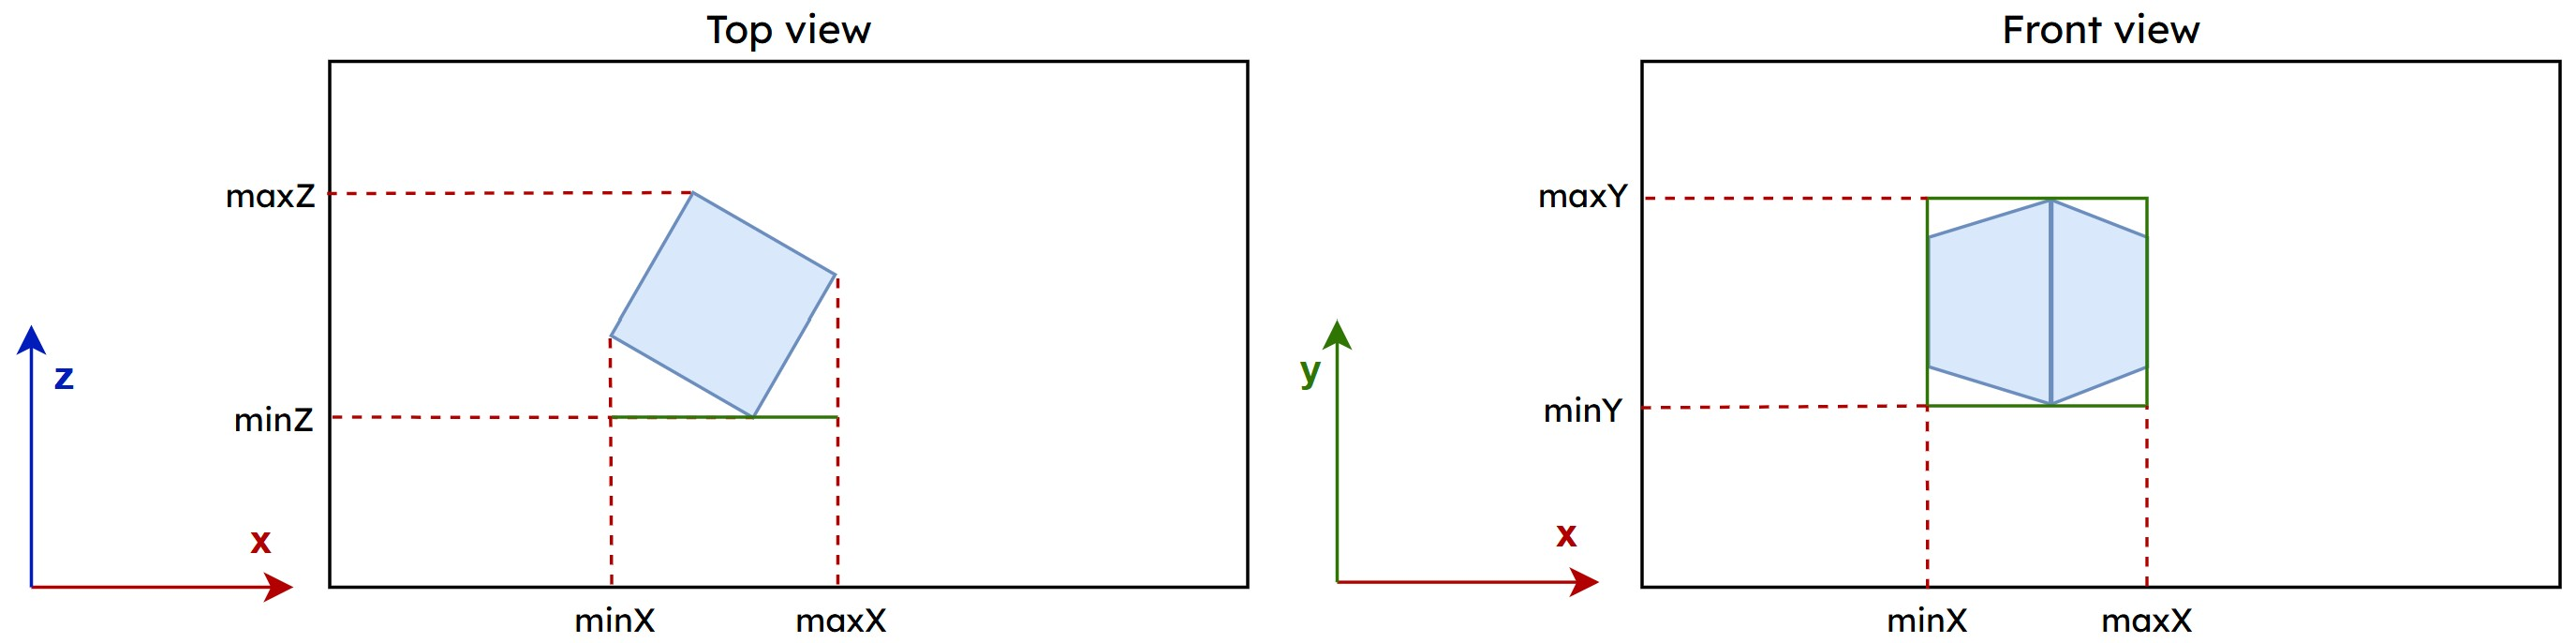
\includegraphics[width=\linewidth]{images/graphics/screen_space_occlusion_test.jpg}
    \caption{The occlusion test is done in screen space using the \emph{min} and \emph{max} boundaries. The octree node 
    is shown in blue, and the respective \emph{min} and \emph{max} values are traced by the dotted red lines. The green 
    line represents the rectangle as viewed from above (left). The same rectangle is shown from a front view as a 
    representation of the octree nodes screen space occupancy (right).}
    \label{fig:screen-space-occlusion-test}
\end{figure}

\noindent
Now the hierarchy is traversed until the node is found to be fully occluded or until the hierarchy is fully traversed 
and the node is found to be visible. Note that the area that is checked is not perfectly congruent with the actual 
projected boundary box. This can lead to edge cases, where a few octree nodes are drawn, although they are actually 
completely occluded. Still, this algorithm is completely conservative, meaning that it does not occlude any geometry 
that should in fact be visible.

\begin{figure}[h]
    \centering
    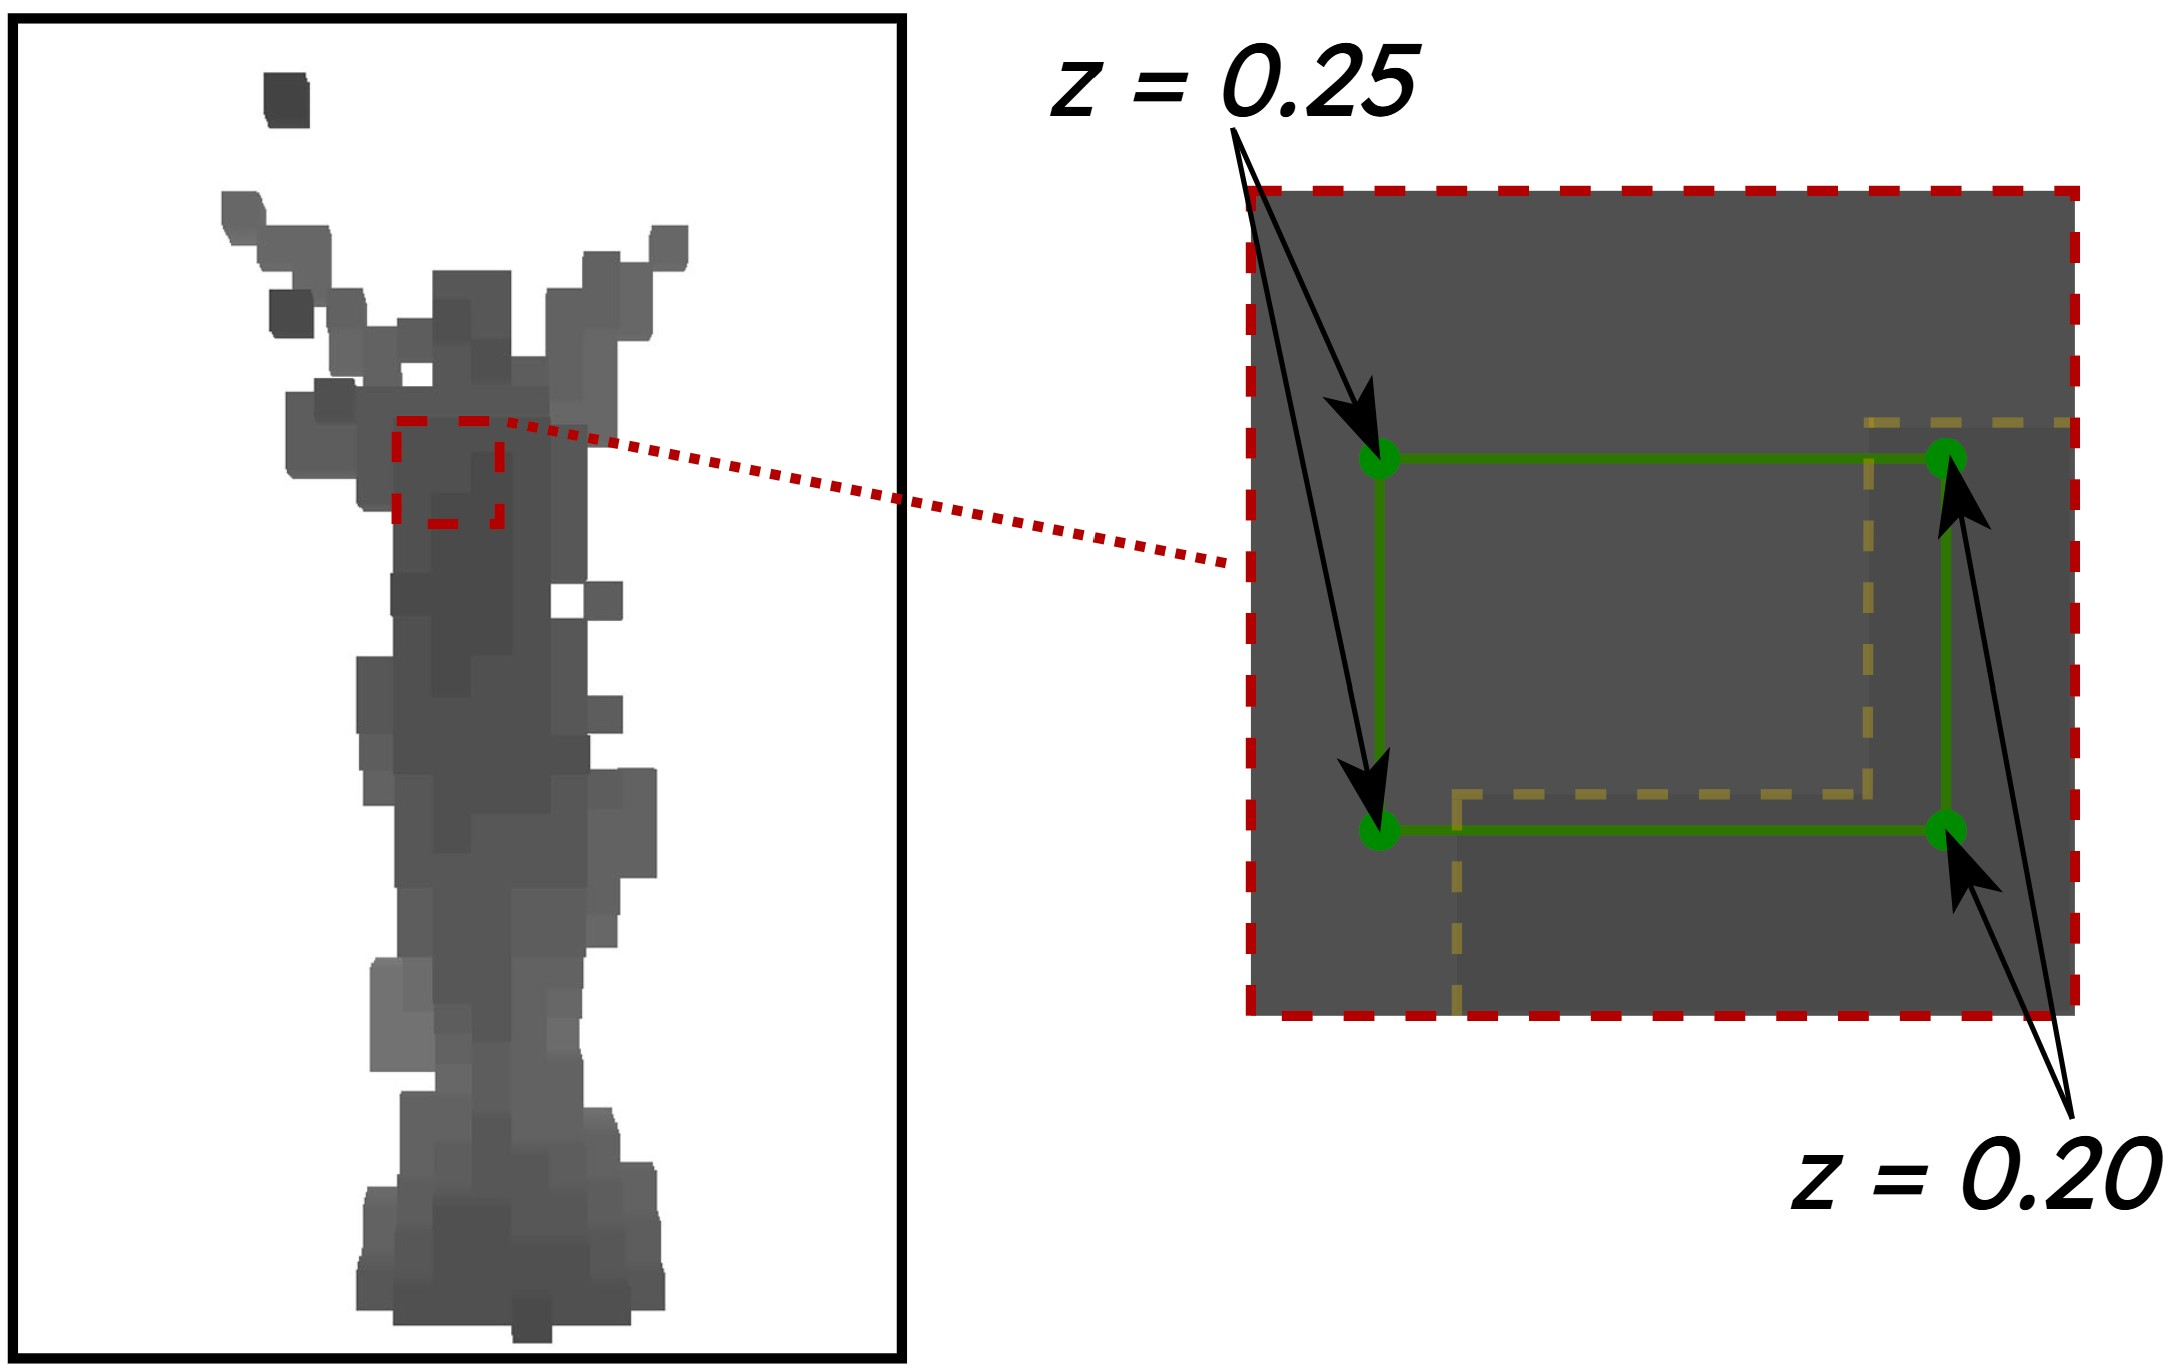
\includegraphics[width=\linewidth]{images/graphics/visibility-hiz-sampling.jpg}
    \caption{The \ac{HiZ} pyramid being sampled using the corners of the screen-space rectangle, shown in green. 
    The dotted yellow line resembles the border between different depth values in the buffer. Sampling the four 
    corners can provide up to four different depth values. The smallest one being the "nearest" occluder.}
    \label{fig:visibility-hiz-sampling}
\end{figure}


\noindent
The complete occlusion culling routine computes the bounding box corners as \emph{UV} coordinates so it is independent 
from the mip level the depth values are checked against. In the best case, the visibility can be determined by using 
the coarsest mip level. In the worst case, all mip levels up to the full resolution depth buffer need to be checked.
The routine is shown in listing \ref{lst:occlusion-culling-algo} as pseudocode.

\fbox{
\begin{minipage}{\linewidth}
\begin{algorithm}[H]
\SetAlgoLined
\KwIn{float4 basePosAndScale}
\KwResult{Boolean indicating whether a bounding box is visible}

\SetKwFunction{FMain}{IsVisible}
\SetKwProg{Fn}{Function}{:}{}
\Fn{\FMain{float4 basePosAndScale, Texture2D HiZPyramid}}
{
    float4 center $\gets$ float4(basePosAndScale.xyz, 1.0f)\;
    float scale $\gets$ abs(basePosAndScale.w)\;
    \BlankLine

    float minX $\gets$ GetMinXFromProjectedBoundingBox(center, scale)\;
    float maxX $\gets$ GetMaxXFromProjectedBoundingBox(center, scale)\;
    float minY $\gets$ GetMinYFromProjectedBoundingBox(center, scale)\;
    float maxY $\gets$ GetMaxYFromProjectedBoundingBox(center, scale)\;
    float minZ $\gets$ GetMinZFromProjectedBoundingBox(center, scale)\;
    \BlankLine

    Rect uvRect $\gets$ CalculateUVRect(minX, maxX, minY, maxY, minZ)\;
    \BlankLine

    \For{$mipLevel \gets HiZPyramid.GetNumMipLevels() - 1$ \KwTo $0$}{
        float depthVertex1 $\gets$ HiZPyramid.Sample(uvRect.vertex1, mipLevel)\;
        float depthVertex2 $\gets$ HiZPyramid.Sample(uvRect.vertex2, mipLevel)\;
        float depthVertex3 $\gets$ HiZPyramid.Sample(uvRect.vertex3, mipLevel)\;
        float depthVertex4 $\gets$ HiZPyramid.Sample(uvRect.vertex4, mipLevel)\;
        \BlankLine

        \If{max(depthVertex1, depthVertex2, depthVertex3, depthVertex4) < minZ}{
            \Return{false}\;
        }
    }

    \Return{true}\;
}
\caption{Occlusion Culling algorithm.}
\label{lst:occlusion-culling-algo}
\end{algorithm}
\end{minipage}
}
    
\vspace{0.5cm}


\section{Implementation Limitations}

The implementation features some limitations that need to be considered for the experimental setup 
in the following chapter.\\

\noindent
When dispatching a large amount of data using compute shaders, there are hardware limtiations for 
dispatch numbers in the shader. For the shader model used here, the maximum number of thread groups 
that can be dispatched in one call is $65,536$. For a thread group size of $64$, this results in a 
maximum voxel count of $4,194,304$. This amount of voxels is considered enough for this work but 
might pose a limitation for larger scenes. \\

\noindent
If more voxels are needed, the groupsize can be increased further, which also results in a larger 
octree node size, given that the implementation is similar to the one presented here. Another way 
to increase the total amount of voxels is to draw the scene in multiple passes, invoking the task 
shader more than once.\\

\noindent
Furthermore, the implementation poses some visual errors when viewing the scene from specific 
angles. It is assumed that this might be due to precision errors, but this assumption could not 
be finally confirmed. This problem is, however, managable by shortcutting the \ac{HiZ} pyramid 
and using the full-resolution depth buffer for the visibility test directly, without traversing 
the hierarchy. This results in a functional occlusion culling without visual errors and is used 
for all of the following measurments. \\

\noindent
This modification reduces the time required for traversing the hierarchy. However, since it was 
applied uniformly across all tested configurations, any resulting inaccuracies are eliminated, 
ensuring full comparability between the tested configurations. 
